\documentclass[11pt]{article}
%\documentclass{bioinfo}
\usepackage{epsfig,longtable}
\usepackage{epsfig}
%\usepackage{fullpage,doublespace}
%\usepackage{psfrag}
%\usepackage{genres}
\usepackage{times}
\usepackage{latexsym}
\usepackage{amssymb}
\usepackage{fancybox,subfigure}
\usepackage{floatflt,graphicx}
\usepackage[normalem]{ulem}
\usepackage[reqno]{amsmath}
\usepackage{multirow}
\usepackage{times}
\usepackage{geometry}
\usepackage{algorithmic}
\usepackage{newalg}
\usepackage{lscape}


\geometry{tmargin=1in,bmargin=1in,lmargin=1in,rmargin=1in}
\linespread{0.95} \interfootnotelinepenalty=10000

% Different font in captions
\newcommand{\captionfonts}{\small}
\newtheorem{problem}{Problem}

\makeatletter  % Allow the use of @ in command names
\long\def\@makecaption#1#2{%
  \vskip\abovecaptionskip
  \sbox\@tempboxa{{\captionfonts #1: #2}}%
  \ifdim \wd\@tempboxa >\hsize
    {\captionfonts #1: #2\par}
  \else
    \hbox to\hsize{\hfil\box\@tempboxa\hfil}%
  \fi
  \vskip\belowcaptionskip}
\makeatother   % Cancel the effect of \makeatletter

\setlength{\topmargin}{-0.9in}
\usepackage{latexsym}
\setlength{\columnsep}{0.5cm}
\setlength{\oddsidemargin}{-0cm}
\setlength{\evensidemargin}{-0cm}
\setlength{\textwidth}{6.5in}
\setlength{\textheight}{9.5in}
\newcommand{\old}[1]{}
\newcommand{\match}{\stackrel{M}{=}}
%\newcommand{\ncite}[1]{(\cite{#1})}
\newcommand{\ncite}[1]{$^{\mbox{\tiny \cite{#1}}}$}
%\newcommand{\nncite}[1]{\cite{#1}}
\newcommand{\frags}{{\cal F}}
\newcommand{\snips}{{\cal S}}
\newcommand{\A}{{\tt A}}
\newcommand{\B}{{\tt B}}
\newcommand{\gap}{{\tt -}}
\newcommand{\ideas}{\vskip 0.6cm {\bf IDEAS:\ }}
\newcommand{\motivation}{\vskip 0.6cm {\bf MOTIVATION:\ }}
\newcommand{\mcost}[2]{#1 #2}
\newcommand{\ali}{$\mbox{ }$\hspace{0.2in}}
\newcommand{\acomment}[1]{\hspace{1in}\#{\em #1}}
\newcommand{\beqn}{\begin{equation}}
\newcommand{\eeqn}{\end{equation}}
\newcommand{\comment}[1]{******* {\em #1} *******}
\newcommand{\captionsize}{\footnotesize}
\newcommand{\lpr}{\hspace{0.5pt}\Rsh}
\newcommand{\rpr}{\Lsh}
%%%%%%%%%%%%%% FIGURE within a box
\newenvironment{boxfig}[1]{\fbox{\begin{minipage}{\linewidth}
                        \vspace{1em}
                        \makebox[0.025\linewidth]{}
                        \begin{minipage}{0.95\linewidth}
                        #1
\end{minipage}
                        \end{minipage}}}

\newcommand{\MST}{\ensuremath{\mathit{MST}}}
\newcommand{\dist}{\ensuremath{\mathit{dist}}}
\newcommand{\TG}[2]{\ensuremath{\mathit{#1}^{(#2)}}}
\newcommand{\CC}{\ensuremath{\mathcal{CC}}}
\newcommand{\psubs}{\stackrel{\subset}{+}}
\newcommand{\rs}{\ensuremath{\mathit{R_s}}}

%%%%%%%%%%%%%%%%%%%%%%%%%%%%%  THEOREM-LIKE ENVIRONMENTS

\DeclareMathOperator*{\argmin}{argmin}
\newtheorem{THEOREM}{{\bf  Theorem}}
\newenvironment{theorem}{\begin{THEOREM} \hspace{-.85em} {\rm :} \rm}%
                        {\end{THEOREM}}
\newtheorem{LEMMA}[THEOREM]{Lemma}
\newenvironment{lemma}{\begin{LEMMA} \hspace{-.85em} {\bf :} \rm}%
                      {\end{LEMMA}}
\newtheorem{COROLLARY}[THEOREM]{Corollary}
\newenvironment{corollary}{\begin{COROLLARY} \hspace{-.85em} {\bf :} \rm}%
                          {\end{COROLLARY}}
\newtheorem{PROPOSITION}[THEOREM]{Proposition}
\newenvironment{proposition}{\begin{PROPOSITION} \hspace{-.85em} {\bf :} \rm}%
                            {\end{PROPOSITION}}
\newtheorem{CLAIM}[THEOREM]{Claim}
\newenvironment{claim}{\begin{CLAIM} \hspace{-.85em} {\bf :} \rm}%
                      {\end{CLAIM}}
\newtheorem{OBSERVATION}[THEOREM]{Observation}
\newenvironment{Observation}{\begin{OBSERVATION} \hspace{-.85em} {\bf :} \rm}%
                      {\end{OBSERVATION}}
\newtheorem{DEFINITION}{Definition}
\newenvironment{definition}{\begin{DEFINITION} \hspace{-.85em} {\bf :} \rm}%
                           {\end{DEFINITION}}
\newcommand{\QED}{\hfill$\Box$ \vskip 0.1cm}
\newenvironment{proof}{\noindent {\bf Proof:} \hspace{.677em}}{\QED}

\newcommand{\inspect}{${\rm Inspect}$}
\newcommand{\vargroupingthresh}{variant distance threshold}



\begin{document}

% \title{Relative Quantification and False Discovery Rates of Isobaric Modified Peptide Variants}
\title{False Localization Rates for Site Assignment of Post-Translational Modifications}


\date{}
\maketitle

\begin{abstract}
Accurate identification of post-translational modification (PTM) sites by tandem mass spectrometry (MS/MS) remains a major challenge in proteomics. While peptide identification has become largely automated, PTM site assignment often requires substantial manual curation and experimental follow up. Statistical validation of peptide identifications is commonly done using False Discovery Rates (FDR). The lack of an equivalent method for assessing False \emph{Localization} Rates (FLR) has made it difficult to easily validate reported PTM localizations from mass spectrometry experiments. Current approaches localize PTMs using fixed score thresholds and do not enforce FLR on high-throughput searches. We propose one of the first generic approaches for calculating FLR using assignments of PTMs to incorrect residues as decoys while hits to valid residues as target. We also introduce a new scoring function which is able to explicitly model ambiguous or partially-localized PTMs and for co-elution of differently-modified variants of the same peptides with the same PTMs on different sites. We demonstrate our approach on MS/MS spectra on synthetic human phosphopeptides, Human lens, whole lysate with a diverse set of PTMs and high throughput \emph{Saccharomyces  cerevisiae}  phosphopeptides where we are able to localize approximately 19\% more MS3 and 33\% MS2 spectra than Ascore.
%We validate our approach on MS/MS CID spectra from synthetic human phosphopeptides and human lens whole lysate with a diverse set of PTMs and high throughput \emph{Saccharomyces  cerevisiae}  phosphopeptides. 

%One of the common limitations of mass spectrometry-based techniques in PTM identification is co-elution of different positional PTM variants with similar mass and retention times resulting in \emph{mixture} tandem mass spectrum. In this study, we propose a novel computational framework to accurately identify and quantify co-eluting peptide modification variants. Our approach utilizes the presence and absence of fragment ions in MS/MS data as well as some intrinsic properties of fragment ions, \emph{detectabilities}, that cause the variability in the observed peak intensities. We either report a precise site for modification or a mixture of modification variants with accurate relative abundances along with the ambiguities in the site assignment if there is no/little evidence in the tandem mass spectrum.
%
%For evaluation of our quantification results on a MS/MS dataset, we propose a novel target-decoy FDR strategy to measure error rate in PTM site assignment. This strategy allows us to control the FP rate in PTM identifications. We have demonstrated the robustness of our framework on a human lens dataset with a number of different PTMs. At an estimated $<2\%$ FDR, we confirm InsPecT�s PTM site assignment for $82.1\%$ of cases. In $13.4\%$ of the cases, InsPecT had the right �region� but the site assignment is actually ambiguous. In the remaining $4.5\%$ of cases, we report a mixture of variants or a site different than Inspect's assignment. In those cases, manual inspection also mostly reveals multiple sites or that InsPecT did not consider the correct site. We validate our framework also on simulated mixtures of up to $3$ variants and report high performance of identification and quantification of variants at $1\%$ FDR.

\textbf{Keywords: } tandem mass spectrometry, post-translational modifications, site assignment, false discovery rate, quantification.

\end{abstract}

\section{Introduction}
Mass spectrometry is the most commonly used approach in high throughput proteomics and the dominant approach for large scale characterization of post translational modifications (PTMs)~\cite{mann03}.  While large scale identification of modified peptides is common~\cite{beausoleil04,dephoure08,Trinidad2012} and appropriately controlled by false discovery rates (FDR), the lack of an equivalent approach for PTM site assignments commonly results in the need for extensive manual validation. Probabilistic scoring methods have reduced the need for extensive manual validation, but still do not offer a global, data dependent measure of the quality of localization results. Similarly to when delta score thresholds were first introduced for database searches for peptide identification, to date the recommended fixed thresholds for site assignment are based upon empirical false localization rates estimated from small sets of synthetic peptides rather than re-estimated for each experiment. Moreover, since fixed thresholds may correspond to varying FLRs on different data, these also do not offer a way to compare competing fixed threshold scoring methods of the same datasets.

For peptide identification, false discovery rates (FDR) are widely used to allow estimation of the false identification rate for entire datasets from any experiment setup~\cite{nesvizhskii10}. PTM localization does not currently have an equivalent data-dependent method~\cite{chalkley12}. A similar FDR approach is necessary for the experiment-wide significance assessment of PTM site assignments. While there have been attempts to approximate FLR using invalid modification amino acid sites for particular modifications as ``decoy'' results, such methods require that the ``decoy" sites appear in similar frequency and in close proximity to the actual modification sites~\cite{Baker2011}. In datasets with a large number of possible modifications (such the human lens dataset used here), this is both impractical to automate and there may not be appropriate ``decoy'' candidates depending on the modification. Delta score approaches such as Mascot Delta Score~\cite{savitski11} and SLIP scores~\cite{Baker2011} take the difference between the top two site assignments and rely on fixed thresholds based on synthetic datasets or the approach described above. Probabilistic score methods such as Ascore~\cite{beausoleil06}, PTM Score (from MaxQuant)~\cite{Olsen2004}, PhosphoRS~\cite{Taus2011}, Phosphorylation Localization Score
(PLScore) in Inspect~\cite{Albuquerque2008}, SloMo~\cite{Bailey2009} and Phosphorinator~\cite{Phanstiel2011} propose to estimate probabilistic scores proportional to the number of site determining peaks between PTM sites. Since these use fixed thresholds which are independent from the dataset, they do not correct for multiple hypothesis testing and do not necessarily result in comparable false localization rates across datasets and experimental conditions.

%talk about ILP from Ben Garcia's group! Actually, maybe not. His work seems to focus on getting all modified forms of a particular peptide based on parent mass. 

Here we propose a new framework for estimation of false localization rates (FLRs) \-- data-dependent false discovery rates for PTM site assignments. First, in contrast to the current methods which assign delta scores between candidate PTM sites, our approach assigns scores to PTM {\em variants} of the same peptide where a variant is defined as a distinct combination of site assignments for the PTMs a particular peptide sequence. Second, we extend the concept of the Target/Decoy Approach~\cite{elias07} where invalid peptide sequences are used to estimate false identification rates against valid peptide sequences and use invalid (decoy) PTM site assignments, such as phosphorylation on Glycine, to estimate false localization rates on valid (target) sites. Third, we allow each MS/MS spectrum to be composed of more than one variant, thus allowing for identification of co-eluting variants and ambiguous and partially-ambiguous PTM site assignments.

%include results!

%In this paper, we propose the first generic approach to estimating false discovery rates (FDRs) for PTM site assignments. We propose a new way to define decoy databases specifically for this purpose, allowing the assignment of FDRs to site-localization score thresholds. In brief, our approach first ignores the knowledge of which residues are valid modification sites (i.e., decoy = invalid PTM sites), assigns a score to every amino acid residue as a putative modification site and then estimates how often each score threshold results in invalid site assignments. Use of this target-decoy based FDR strategy not only helps to control the false hit rate in the site assignments, but also allows us to identify putative novel modification sites.

To demonstrate our FLR framework, we further propose the first variant scoring scheme supporting ambiguity and co-elution and show how spectra of unmodified peptides can be used to assess the reliability of site assignments in spectra of the corresponding modified peptides.
% Our FDR techniques are coupled with a new scoring scheme. 
A variant scoring scheme should be able to distinguish between correct and incorrect PTM site assignments by addressing the challenges inherent to mass spectrometry of peptides: ambiguity due to incomplete MS/MS fragmentation and co-eluting peptides with the same modification on the same peptide sequence but with different modification sites, thus possibly resulting in multiple correct site assignments per spectrum (e.g., as in histone proteins~\cite{DiMaggio2009}). 
%It is crucial to develop a computational approach to determine ambiguity and confidently identify all present modification sites in a tandem mass spectrum with precise site localizations to the extent that MS/MS data allows.
%
Our proposed variant scoring scheme uses linear programming to decompose each MS/MS spectrum into all of its possible variants and assign a separate score to each distinct variant. Ambiguity is then addressed by grouping indistinguishable variants into {\em variant groups} and co-elution is automatically captured by co-occurrence of high-scoring distinct variants in the same MS/MS spectrum.
%
%Here, we also propose a novel computational scoring scheme to peptide site assignments modeling ambiguity and co-elution. Given an MS/MS spectrum, peptide sequence and set of modifications masses we assume that each modification can be associated with every amino acid. We enumerate all possible combinations of modifications and sites (modification variants) and then formulate a linear programming (LP) problem to solve for the relative abundances of each variant. In our LP formulation, we use the expected intensity of fragment ions in MS/MS data to model the . We estimate ion intensities as an intermediate step to our approach and incorporate them in our LP formulation. Another novel aspect of our approach is that we report ambiguities in the assignment of modifications when there is no/little evidence in the MS/MS data for particular variant(s). In other words, we group the variants based on presence or absence of peaks distinguishing between the variants. If two or more variants are indistinguishable with the given data, we report a quantity for the group instead of the individual variants.

The proposed scoring scheme and FLR estimation method was validated by using a set of 180 synthetic phosphopeptides~\cite{savitski11}. The $R^2$ value between the estimated and actual FLR, even for a relatively small dataset was between $.633$ and $.809$ indicating that our method of estimating FLR, especially in cases where there are larger numbers of results, will likely yield a reasonable estimation of FLR. The method also shows improvement over existing delta scoring methods in terms of the number of results localized at the same thresholds. In a high throughput dataset of \emph{Saccharomyces  cerevisiae} phosphopeptides we were able to demonstrate a 19\% increase in localization over ascore in MS3 spectra and a 33\% increase in localization in MS2 over Ascore at a 5\% FLR threshold and an Ascore threshold of 13. In a human lens whole lysate sample with a diverse set of PTMs at an FLR of 5\% we were able to unambiguously localize approximately 50\% of non trivial results and partially localize 60\%  at an FLR of $5\%$ even with 17 types of modifications allowed with up to two modifications per peptide.

\section{Methods}
After identifying spectra using an existing search tool, localization for spectra with PTMs consists of two steps. First, each modification variant (observed modifications and their position on a peptide) is given a score. Next, all modification variants in the entire dataset are sorted based on score and evaluated to estimate the false localization rate (FLR) at different score cutoffs. In the FLR step, all modifications which are assigned to an incorrect amino acid residue are considered invalid. The FLR approach relies on the fact that each possible modification site (even incorrect ones) are evaluated in isolation, so current delta score methods are unsuitable for this method. Our scoring method used for FLR generates scores for each possible modification variant based on how much the theoretical spectra for each variant contributes to the actual modified spectrum. This method of estimation works under the assumption that any particular expected theoretical peak in a particular variant will be scaled by its quantity in the modified spectrum. For example if a variant contributes 50\% to the final spectrum we can expect that each peak intensity in the observed modified spectrum will be 50\% of the predicted intensity for that ion. In this case we use the estimated quantity of each variant as the input score for FLR. Figure~\ref{fig:flowchart} provides an overview of our approach.

Scoring starts with a modified spectra and its associated peptide identification. All possible combinations of the observed modifications on the peptide and the amino acid sites are generated to create the possible modification variants for the peptide. The unmodified version of the peptide identification is then used to find an unmodified spectrum of the unmodified peptide. A theoretical spectra for each variant is then generated from the spectrum of the unmodified peptide by taking the intensity of all identified ions (bs and ys for CID) and shifting the masses by the expected modification mass (note that this shift may be zero depending on the position of the modifications on the modification variant). Given the observed modified spectrum and the theoretical spectra for each variant, the relative abundances of variants are estimated using a linear programming (LP) formulation which estimates the quantity of each variant present in the final modified spectrum by minimizing the error between the observed modified spectrum and the expected intensities based on the quantities of each variant. Finally, we group the indistinguishable modification variants based on the modified spectrum. When there are no or very few peaks distinguishing two modification variants in the mixture spectrum, it is impossible for LP to differentiate between the two variants as well. In such cases, the individual variant abundances are not accurate but rather the summed abundance for the group. We output the relative abundances of variant groups instead of individual variant groups. 

Following scoring, a target-decoy strategy is adopted to determine the global FLR for site assignments. The knowledge of site-specificity of the modification is introduced at this point. The variant groups which assign each PTM to at least one valid site are valid and are added to the target database. In cases with multiply modified peptides, all PTMs must have at least one valid site assignment in order to be considered valid. Similarly, variant groups which assign any PTM to invalid sites only are considered invalid and added to the decoy database. Each variant group is then scored by the total estimated abundance. FLR is then computed at each score threshold by estimating how often that threshold results in invalid/decoy site assignments. The grouping threshold can affect the ambiguity of results and the number of results output at different FLR cutoffs, so an alternate method to choosing a fixed cutoff is to choose successive grouping thresholds and calculating FLR at each threshold (See Section~\ref{sec:FLR}).

In the following subsections, we will discuss building the LP and grouping variants in more detail.

\begin{figure}[]
\centering % trim=l b r t
\includegraphics[height=0.7\textwidth]{fig/intro.pdf}
\caption{\small Overview of FLR approach: a) All modification sites are scored individually. b) Invalid site assignments are used as decoys for TDA-like calculation of FLR.\\ (a1) For each modified spectra, the first step in PTM localization is scoring the modification variants. The modified spectrum is modeled as a mixture of the theoretical spectra of the modification variants. By evaluating the contribution of each theoretical spectrum to the modified spectrum, the quantity of each variant can be estimated through linear programming (LP). (a2) Ambiguities in site assignment are handled by grouping indistinguishable sites into variant groups. Due to missing peaks in the modified peptide spectrum, some variants are indistinguishable in the LP. In such cases, we report the total abundance for the site groups instead of the abundance of the individual sites. (b1) A target-decoy strategy is adopted to determine the global FLR for site assignments. The knowledge of site-specificity of the modification is introduced at this point. The variant groups which assign each PTM to at least one valid site are valid and are added to the target database. Variant groups which assign at least one PTM to invalid sites only are invalid and added to the decoy database. Each variant group is then scored by the total estimated abundance. FLR is then computed at each score threshold by estimating how often that threshold results in invalid/decoy site assignments. (b2) PTM site assignments at a chosen FLR are reported as output. If the peptide has one reported group with one valid site only, then the modification is unambiguously assigned to that valid site. If the reported group has more than one possible valid site but does exclude sites, this is considered partially localized. If the reported group has multiple valid sites, then the site assignment is ambiguous. If the reported group contains all possible variants, we consider this as a non-localized result. Multiple groups passing the score threshold for the peptide are an indication of co-elution where the relative scores can be interpreted as the relative abundances of the co-eluting sites.}
\label{fig:flowchart}
\end{figure}


\subsection{Enumeration of Modification Variants}\label{sec:enumerationOfVariants}
Once a search has been performed and a particular spectra has been identified as containing PTMs, all modification variants must be generated to be scored by LP. Each variant of a peptide consists of the same  sequence and modifications, the only difference is in the location of the modification types. At most one modification mass is allowed on each amino acid; multiply-modified amino acids are modeled using modifications of the resulting aggregate mass. For example, di-methylation is represented using nominal mass 28 Da instead of two methylations, each of mass 14 Da. Note that at this stage modification site specificity is ignored and all possible amino acid sites are considered candidates for modification. Given a peptide identification of length $n$ and consisting of the multiset of modification masses $\mathcal{M}={m_{1},\cdots,m_{k}$ with $d$ duplicate masses, there are $\binom{n}{k} \cdot \frac{k!}{d!}$ possible modification variants. 

The modification variants are exhaustively enumerated by generating all distinct permutations of length $n$ consisting of $k+1$ elements (k modifications with a placeholder element for unmodified positions).

\subsection{Inference of Fragment Ion Intensities}\label{sec:inferDetectabilities}
Consider a fragment ion of a peptide. We make the assumption that the
intensity of an ion remains constant, even when the peptide is
modified. This assumption is borne out by empirical observation of conservation
of spectral shapes of a peptide sequence across different unmodified
and modified tandem mass spectra. Previously, Sniatynski et
al.~\cite{Sniatynski2006} showed that delay-series
correlation between the mass spectra of modified and unmodified
peptides revealed significant spectral overlap at an offset indicative
of the modification. Others, including us, make a similar
observation~\cite{bandeira07pnas}.

We observe similar behavior in our test MS/MS datasets. We measure the similarity between two spectra
using dot product (cosine score) which is a widely accepted measure for
spectral similarity.~\cite{lam07,Stein1994} For the purposes of this method, extracted ions are used so that like ions are compared with each other rather than comparing by mass windows. For example intensities of a modified b2 ion is compared to its unmodified b2 counterpart in a different spectrum. For simplicity, we define theoretical peptide masses $Masses(P)$ as the set of theoretical prefix and suffix masses from $P$ based on its amino acid sequence. Since in this case, we only consider collision induced dissociation (CID) MS/MS, $Masses(P)$ consists of b and y single and doubly charged and b and y isomers with an extra dalton. However, depending on the dissociation method used, this can be easily configured to support other ion types. See Section~\ref{sec:inferDetectabilities} for more details. 

\begin{enumerate}
\item Given a spectrum $S$ from a peptide $P$, we define $Intensities(S,P)$ as the intensities of the spectrum peaks in $S$ at $Masses(P)$. Without loss of generality, the vector $Intensities(S,P)$ is always normalized to Euclidian norm 1.
\item Given a spectrum $S$ from a peptide $P$ and a spectrum $S_v$ from a modified peptide variant $P_v$, we define the similarity between the extracted peak intensities as

    \begin{eqnarray*}
    Similarity(S,S_v) & = & \cos(Intensities(S,P),Intensities(S_v,P_v)) \\
                      & = & Intensities(S,P) \cdot Intensities(S_v,P_v)
    \end{eqnarray*}
\end{enumerate}

In Supplemental Figure~\ref{fig:CosineScoreDist}a, we show the distribution of the cosine score similarities of unmodified charge 2 human lens spectra pairs which are identified as the same peptide. $99.44\%$ of the pairs have more than $0.4$ cosine similarity confirming that the fragment ion intensities are conserved across unmodified spectra. The distribution of spectral similarities of modified-unmodified spectra pairs is shown in Figure~\ref{fig:CosineScoreDist}b. We see that even after modification, there is a significant spectral overlap between the spectra pairs of the same peptides: $96.2\%$ of the pairs shows more than $0.4$ cosine similarity. By contrast, as shown in Supplemental Figure~\ref{fig:CosineScoreDist}c, for unmodified spectra of the same length with parent masses within 20 Da of each other, only $65.8\%$ of the spectra are above a cosine of $0.4$.

Even for phosphorylation, which is known to strongly affect CID fragmentation~\cite{Tholey1999,Moyer2002}, this assumption seems to hold. For MS2 data in Supplemental Figure~\ref{fig:Yeast_CosineScoreDist}b, $94.98\%$ are above cosine .4. For unmodified vs modified MS3 data, shown in Supplemental Figure~\ref{fig:Yeast_CosineScoreDist}c over $89.5\%$ of spectra are above .4.

In cases where the unmodified spectrum is not available in the experiment itself, we can either use spectral libraries ~\cite{speclib_nist_human_yeast} or a prediction tool such as MassAnalyzer ~\cite{zhang04,zhang05,zhang10}. From these sets of unmodified spectra and identified spectra within the dataset used, the best candidate unmodified spectrum for a particular modified spectrum is chosen. For a modified spectrum $S'$ annotated by $P'$, we choose all spectra associated with the unmodified peptide $P$ of the same sequence. If there is more than one candidate spectrum, we choose the unmodified spectrum with the highest cosine to the modified spectrum as our unmodified spectrum $S$. Note that there are other methods for choosing the best candidate, for example, giving preference to unmodified spectra from the same dataset as the modified spectrum. See Supplemental Materials \ref{sec:inferDetectabilities} for more details.

Following the selection of the best candidate spectrum, the theoretical spectrum for each variant is generated from the unmodified peak intensities.

\begin{enumerate}
\item Given a spectrum $S$ from an unmodified peptide $P$, we want to predict a theoretical spectrum for $P_v$, a modified variant of $P$.
\item Extract peak intensities from $S$ at $Masses(P)$ and use these to set the corresponding peak intensities in $S_v$ at $Masses(P_v)$.
\end{enumerate}

\subsection{Quantitation of Modification Variants via Linear Programming}\label{sec:quantificationLP}
An experimental spectrum is modeled as a linear combination of the theoretical spectra for all possible variants of the same modified peptide sequence. By scaling peaks in each modification variant's theoretical spectrum based on the observed peaks in the modified spectrum, we can estimate the overall quantity of each modification variant using linear programming.

For a modified spectrum $S'$ with a peptide identification $P'$ with the unmodified peptide version of $P$, all variants are generated as described in Section~\ref{sec:enumerationOfVariants}. In order to build the LP, all possible theoretical peak masses for every variant need to be generated. The multiset of modifications $\mathcal{M}$ is extracted from $P'$. All possible combinations of $\mathcal{M}$ are generated and summed together to find all distinct mass shifts for unmodified peaks in the spectrum. All peaks from $Masses(P)$ are then added to the theoretical ion vector $T$. All modification mass shifts are also added to each peak in $Masses(P)$ and added to $T$. 

\begin{enumerate}

\item For each theoretical ion $t_j$ in $T$, if a peak with intensity $y$ from $S'$ is within the expected peak tolerance, then observed peak intensity $O_j = y$ otherwise observed peak intensity $O_j = 0$.

\item For each theoretical ion $t_j$, if there is a variant $v_i$ where $t_j \in Masses(v_i)$ in the expected peak tolerance, assume that $Q_i$ is contributing to overall intensity $O_j$. We add all such variants to $\mathcal{V}_j \subset V$. The expected intensity of the peak theoretical peak $t_j$ is determined as described in Section\ref{sec:inferDetectabilities} and designated as $d_j$. 

For each theoretical ion, it is assumed that the observed peak is the sum of the contribution of all variants scaled by their quantity and expected intensity.

\[
O_j \approx \sum_{i=1}^{|\mathcal{V}_j|}  d_j \times {Q_i}
\]

From this, the error of each peak can be approximated as follows

\[
\epsilon_j = O_j - \sum_{i=1}^{|\mathcal{V}_j|} d_j \times{Q_i}
\]
\end{enumerate}

An LP is then generated which minimizes the error of each peak.

\[
\begin{array}{l|l|l}
{\rm Input} & {\rm Output} & {\rm Formulation} \\
\hline
\begin{array}{l}
d_j \mbox{ for every ion } j \\
O_j \mbox{ for every ion } j \\
\end{array}&
\begin{array}{l} Q_i \mbox{ for every}\\
\mbox{variant } v_i \\
\end{array}&
\begin{array}{cll}
\min &{\displaystyle \sum_{j=1}^{r}{|\varepsilon_j|}}\\[1.5em]
%{\rm s.t.} & \sum_{p_j\in P} Q_i = 100 & \\[1.5em]
{\rm s.t.}&{\displaystyle \varepsilon_j = O_j - \sum_{i=1}^{|\mathcal{V}_j|} d_j \times{Q_i} }\\
[1.5em]
&{\displaystyle Q_i\geq 0} \\
\end{array}\\
&&\\
&&Q_is\mbox{ are normalized prior to output so that } \sum_i(Q_i) = 1\\
\end{array}\\
\]

Essentially, for each peak we seek to estimate how much each variant contributes to the overall abundance
of that peak based on the expected intensity. We minimize error by comparing this predicted intensity to the modified spectrum. As a simple example, if we have a set of variants (P,16)EPT, P(E,16)PT, PE(P,16)T and PEP(T,16) we expect the $b3$ ion to have an intensity based on the intensity of the $b3$ ion from our unmodified spectrum. The $b3+16$ ion would be contributed to by the expected quantities of (P,16)EPT, P(E,16)PT, PE(P,16)T while the unmodified $b3$ ion would only be contributed to by PEP(T,16). If we do not see the unmodified version of the $b3$ ion and it is strong in the unmodified spectrum, it is likely that the PEP(T,16) variant is not present. We estimate the quantities of all three variants based on the intensities of the modified and unmodified versions of $b3$ and the other ions we observe and try to minimize the difference between our expected intensities and our actual $b3$ intensities. See Supplemental Materials ~\ref{sec:quantificationSupplemental} for more details.

As we have linear constraints, and linear objectives, we can solve the
problem efficiently using existing Linear programming techniques.~\cite{Dantzig1998}
We are able to leverage existing LP solvers such as GLPK \footnote[1]{http://www.gnu.org/software/glpk/} and CPLEX \footnote[2]{www.ibm.com/software/integration/optimization/cplex-optimizer/
} by using the generic CPLEX LP format to formulate our problem.

\subsection{Grouping Modification Variants}\label{sec:groupVariants}
The LP outputs an estimated abundance per modification variant. However, depending on the completeness of the fragmentation pattern, there might be no or very few \emph{distinguishing peaks} between two modification variants. In that case, it is impossible for LP to distinguish between the variants in its abundance assignment. In the absence of distinguishing ions, some estimates for individual variant(s) will not be accurate, but for the \emph{groups} of indistinguishable variants. Therefore, we group these variants that do not have enough/any distinguishing peaks in between, and report total estimated abundance per variant group instead of individual variants. 

In order to minimize the effect that the order of grouping has on the groups which are output, a form of hierarchical clustering is used which recalculates the distance between groups every time pairs of groups are merged.

\begin{enumerate}
\item Form $n$ clusters containing a single variant, $g_{1} \cdots g_{n}$.
\item Find the distance between pairs of variant groups. To calculate the distinguishing intensity between $g_{i}$ and $g_{j}$ we consider all peaks identified by any variant in $g_{i}$ and all peaks identified by any variant in $g_{j}$. If a peak in $S'$ is identified by any variant in $g_{i}$ and not by any variant in $g_{j}$ we add that to the total distinguishing intensity. We then calculate the distance by dividing the sum of distinguishing intensity by the total identified intensity.
\item Find the two groups $g_{i}$ and $g_{j}$ with the lowest distinguishing intensity. If these groups have a distinguishing intensity above our grouping threshold, stop.
\item Merge the $g_{i}$ and $g_{j}$ and create new group $g_{k}$. $Q_k$ is defined as the sum of $Q_i$ and $Q_j$.
\item Recompute distances between $g_{k}$ all other groups.
\end{enumerate}

Grouping variants allows us to report ambiguous site identification of modifications when it is impossible to distinguish between the sites by the detected peaks in the spectrum. A higher grouping threshold will lead to more ambiguous results, while a lower grouping threshold will increase the granularity of the results, but will increase the number of false hits. As we can see in Figure ~\ref{fig:ambiguityVsGrouping}, this threshold can have a very strong effect on the results which is highly dependent on the dataset. Successive thresholds can be used to avoid this problem as described in Section~\ref{sec:FLR}.

Note that this grouping method is only suitable for cases where there are a small number of modifications per peptide. As the number of modifications per peptide increases, there is a combinatorial explosion in the number of possible variants, much like the explosion in search space in peptide database search when more modifications are allowed per peptide. Since hierarchical clustering is essentially an n by n comparison of all the modification variants, this quickly becomes intractable. There are possible ways to address this problem in the future, including dynamically generating variants by iteratively grouping successive positions which do not have distinguishing intensity between them. Such methods will need to be investigated to address localization for highly modified peptides.

\subsection{Evaluation of Dataset Results using FLR}\label{sec:FLR}
In peptide identification, to evaluate the performance of search algorithms on a dataset, use of target and decoy databases is widely practiced. The target-decoy search strategy permits an impartial assessment of search results and by applying a score cutoff, the false discovery rate (FDR) can be controlled at a desired level. We adopt a similar target-decoy strategy to determine the global false-discovery rate (FDR) for modification variant identifications.

In order to calculate FLR, we take groups of variants and their associated quantities. During all previous scoring, amino acid site specificity has been ignored. At this stage we reintroduce the ``known" amino acid specificity for the modification types. These variant groups construct our target and decoy database as we quantify variant groups instead of individual variants. A ``valid variant" has all associated modifications associated with a valid amino acid residue. For example, $(P,42)EP(T,80)IDE$ is a valid variant if we consider n-term acetylation and phosphorylation, $(P,42)E(P,80)TIDE$ would not be a valid variant. If a group has at least one valid variant, it is called \emph{valid group} and it is added to the target. If a group does not have any valid variant, it is an \emph{invalid group} and added to the decoy. Thus, an invalid group is considered a decoy identification while an valid group identified is considered a target identification.

The ratio of target to decoy will be influenced by which modifications are being considered and what their target amino acids are. In order to account for this, we adjust the incorrect hits by a scaling factor. We take the fraction of all valid groups, $TP$ divided by fraction of invalid groups, $FP$ from all of the returned variant groups, even those with a score of 0. This is our scaling factor $\rho$. FLR is determined by taking the number of incorrect hits $I$ and correct hits $T$ and calculating $\frac{I*\rho}{T}$.

FLR estimation by target-decoy strategy is coupled with our scoring scheme. Each instance in target and decoy is assigned a score. In our target-decoy approach for FDR, we use the estimated abundances assigned by LP to score each variant group along with the cosine of the theoretical spectra from our LP output to our original modified spectrum $S'$. This is a reasonable choice since we would have more confidence in the presence of a group if its estimated abundance is high. If the estimated abundance is low, it is more likely that the abundance is assigned due to contaminant peaks or noise. However, the granularity of scoring if only quantity is used is low. Most abundances are at 1 or 0 since the LP is able to unambiguously determine the site. This does not take into account the overall quality of the spectrum, such as a low number of peaks or a large number of low intensity peaks. In order to add an extra layer of granularity we sort by cosine between the estimated theoretical spectrum (based on the calculated quantity of the variant groups and the expected intensities of all theoretical peaks) and the modified spectrum. 

Since variants which do not have enough distinguishing intensity are grouped together, there is another parameter that can affect the results: grouping threshold. If a high threshold is chosen, there will be fewer decoy results, but at the cost of higher ambiguity. (See Figure~\ref{fig:ambiguityVsGrouping}) In order to simplify the handling of grouping thresholds, we use a modified approach when calculating FLR. Instead of picking a static grouping threshold and calculating FLR at that single threshold, we use successive thresholds to maximize the granularity of results while still returning a high number of results.

First, FLR is calculated at the lowest grouping threshold. Then all results above our FLR cutoff are returned. Then for the next threshold, all spectra and their associated variants which were above are cutoff are removed and FLR is recalculated on the remaining set (including recalculating the scaling function). This continues until there are no more grouping thresholds to pass. As shown in Figure ~\ref{fig:ambiguityVsGrouping}, this maximizes the number of results at every FLR threshold. Lower FLR thresholds will push towards more ambiguous results since higher grouping thresholds must be used to maintain that FLR, but this still yields much more robust results than simply picking a static threshold. 

\begin{figure}[h]
\centering
\includegraphics[scale=.9]{fig/ambiguity_vs_grouping.png}
\caption[Hierarchical grouping thresholds vs ambiguity]{This figure illustrates the effect of adjusting grouping thresholds and our FLR on the proportion of total results and what percentage of those results are considered ambiguous. Decreasing the FLR threshold increases the number of ambiguous results as results with more variants grouped together are more likely to include a valid site. Increasing the grouping threshold increases the number of results at every threshold, but includes more ambiguous results. Using successive grouping thresholds means ambiguity is solely affected by FLR and the number of results at every threshold is maximized. Colored portions of each circle indicate the percentage of total results which are considered ambiguous by excluding any valid sites. a) Charge 2 MS2 phosphorylation data b) Charge 2 MS3 phosphorylation data c) Charge 3 MS2 phosphorylation data d) Charge 3 MS3 phosphorylation data e) Charge 2 MS3 lens data f) Charge 3 MS2 lens data}
\label{fig:ambiguityVsGrouping}
\end{figure}

\section{Results}\label{sec:results}
\subsection{Site Assignment Analysis on Synthetic Human Phosphoeptide Dataset}\label{sec:mascotsynthetic}

In this section, we validated our approach on an MS/MS dataset of peptides with known modification sites~\cite{savitski11}. For our analysis we used the LTQ-Orbitrap XL CID data. Full scan MS spectra were acquired in the Orbitrap at a resolution of $60,000$ at m/z $400$ after accumulating ions to a target value of $1*106$. The five most intense ions were selected for fragmentation by CID with a resolution of $.5$ Da for fragment tolerance . These $7,992$ CID spectra were then searched using \inspect ~\cite{tanner05} with $2$ Da parent and $.5$ fragment tolerance against the $153$ proteins from which the $180$ peptides were synthesized plus $8$ common contaminant proteins at a cutoff of $1\%$ FDR. $966$ charge 2 spectra and $281$ charge 3 spectra were identified.

In order to ensure the presence of an unmodified version of each modified peptide, the NIST human ion trap spectral library was included.~\cite{speclib_nist_human_yeast}. MassAnalyzer was also used to generate predictions for the unmodified versions of the modified peptides~\cite{zhang04,zhang05,zhang10} at the appropriate charge states as well.

The identified spectra were then scored using the LP scoring method described above. Peptides which were originally identified by {\inspect} as having a modification on serine or threonine were assumed to have a modified fragment shift of $-18$ ($\beta$ elimination of phosphate)~\cite{Groenborg2002}. Those which were identified as having a modification on tyrosine were assumed to have a modified fragment shift of $+80$~\cite{Steen2001}. These results were then grouped as described in Section~\ref{sec:groupVariants} using thresholds from $.015$ to $.45$ and steps of $.03$. FLR was then applied at successive thresholds as described in Section~\ref{sec:FLR} assuminng that modifications of $-18$ on serine and threonine were valid and modifications of $+80$ on tyrosine were valid.

Based on the empirical FLR of this dataset we were able to compare our expected FLR values. All results at a particular threshold with at least one valid variant were considered. Any valid variant in a particular spectra which had the expected modification site as based on the original synthesis information was considered a target, an incorrect assignment was considered a decoy. As shown in Figure~\ref{fig:syntheticEmpiricalvsEstimated}, for charge 2 data, the estimated FLR are close to the empirical FLR values. In charge 3, the estimated values do not match as well, most likely due to the fact that there were many many fewer results. In addition, there were a number of replicates of the same peptide which may have been a spurious misidentification. (See Appendix~\ref{sec:highScoringDecoyCharge3}). If we discard this specific case, the numbers for empirical and estimated FLR seem to be within a reasonable range of each other.

Even though this is a relatively small dataset, it is clear that FLR combined with our scoring system can provide a good approximation to the empirical FLR for phosphorylated data.

\begin{figure}[h]
\centering
\includegraphics[scale=.5]{fig/synthetic/all_charge_cid_empirical_vs_estimated_flr.png}
\caption{Empirical FLR based on expected residues vs. estimated FLR for the non decoy synthetic results. Only results which were either identical or superstrings of the expected peptide sequence from the original study were considered.  For charge 2 nonunique spectra, the maximum number of results considered at $.09$ FLR were $956$ spectra out of $966$ modified spectra identified by Inspect. The charge 3 nonunique spectra had a maximum number of results of $252$ out of $281$ identified by Inspect. The filtered charge 3 nonunique spectra have Pep0001 A11 filtered. The maximum number of filtered results considered were $245$. }
\label{fig:syntheticEmpiricalvsEstimated}
\end{figure}

\subsection{Site Assignment Analysis on Yeast Phospho-Peptides}\label{sec:yeastphosphoresults}
Next, a discovery study was done on a larger dataset of phospho-peptides in order to to evaluate how well the LP and FLR combined approach approach performs for high throughput phosphorylation site assignment versus current methods such as Ascore~\cite{beausoleil06}.

\begin{figure}[h!]
\centering
\includegraphics[scale=.65]{fig/venn_diagrams.png}
\caption[Ascore vs. FLR in Phosphorylation Results]{Ascore vs. FLR for non-trivial phosphorylation results. Non-ambiguous are FLR results which return only one valid variant. Partially localized results exclude possible valid sites, however there is more than one valid variant. Ambiguous does not exclude any valid site, however, it does exclude incorrect variant sites. Non-localized by FLR means that all possible variants are in one group, no valid or invalid sites are excluded. Non-localized results are included as Ascore only as we do not return any localization information. An FLR cutoff of .05 and an Ascore cutoff of 13 was used. a) Charge 2 MS2 results out of $13,881$ nontrivial results identified by {\inspect}. $13,412$ were below our FLR cutoff, $10,420$ were above the Ascore cutoff. b) Charge 2 MS3 results out of $1,830$ nontrivial results identified by {\inspect}. $1,817$ results were below FLR cutoff, $1,565$ results were above Ascore cutoff. c) Charge 3 MS2 results out of $7,797$ nontrivial {\inspect} results. $6,823$ were below FLR cutoff, $4,824$ were above Ascore cutoff. d) Charge 3 MS3 results out of $760$ nontrivial {\inspect} results. $737$ results were below FLR cutoff, $573$ were above Ascore cutoff.}
\label{fig:ascoreVsLP}
\end{figure}

The dataset consists of both neutral loss dependent MS3 spectra and MS/MS spectra of the de-phosphorylated peptides to increase the likelihood of having unmodified versions of modified peptides from the same dataset. The sample from S. Cerevisiae was first IMAC-enriched for phospho-peptides and neutral loss dependent MS3 spectra were acquired from the first half of the sample. The second half of the sample was CIP treated for removal of the phosphate group, HILIC fractionated into 11 fractions and MS/MS were acquired on the de-phosphorylated peptides. The CIP treated samples also were treated with SILAC K+8 and R+10 modifications. {\tt where is the citation for this? }

% Statistics:
% 152,015 spectra identified, 105,951 identified as charge 2 peptide
% 75,491 unmod peptides, 14,749 unique unmodified peptide,
% 30,460 modified, 7,934 dehydrated, 2,190 unique dehydrated peptide
% 613 modified MS3 peptides have their unmodified version identified
The $1,669,605$ MS2 and $78,939$ MS3 spectra were identified using {\inspect}~\cite{tanner05}, against the Saccharomyces Genome Database from February 2011~\cite{Cherry2012} with parent mass tolerance $2$ Da and fragment mass tolerance $0.5$ at a $1\%$ spectrum level FDR allowing for one phosphorylation or -18 per peptide. The data were searched twice, once with unmodified K and R and once with K+8 and R+10 fixed modifications. Since localization of the SILAC modifications do not matter, fixed mods were used to increase the total number of identifications without significantly increasing search time. In total, $139,628$ spectra were annotated. From these results, $30,292$ modified spectra (excluding those with SILAC mods) were found of which $19,481$ were charge 2 and $10,218$ of which were charge 3. From the MS2 spectra, $4,496$ phosphorylated peptides were identified (ignoring modification position), $927$ of which also were identified in an MS3 spectrum. 

Although the CIP treated sample contained many unmodified versions of the modified peptides, the NIST yeast ion trap spectral library was included in order to capture cases where the unmodified peptide was not identified~\cite{speclib_nist_human_yeast}. Also, for the $4,496$ unique modified peptides, MassAnalyzer was used to generate predictions~\cite{zhang04,zhang05,zhang10} at the appropriate charge states.

The identified spectra were then scored using the LP scoring method described above. Due to some unmodified results having SILAC modifications, altered values for K and R were used on some unmodified spectra. Phosphorylated peptides were assumed to have a modified fragment shift of $-18$ ($\beta$ elimination of phosphate)~\cite{Groenborg2002}.\footnote{Due to the relatively small number of tyrosine phosphorylations (320 total), no special provisions were made to use +80 fragments for tyrosine phosphorylated peptides} These results were then grouped as described in Section~\ref{sec:groupVariants} using thresholds from $.015$ to $.45$ and steps of $.03$. FLR was then applied at successive thresholds as described in Section~\ref{sec:FLR} with the variant groups marked as valid if they assigned the modification to an S or T.  

In order to compare with existing methods, Ascore~\cite{beausoleil06} was run on the phosphorylation data as well. By taking results from {\inspect} and translating into pepxml, Ascore was run using the same input results as our FLR formula.\footnote{We were unable to perform a similar comparison with the lens dataset since Ascore was incorrectly allowing for modifications on serine and threonine for all modification types regardless of whether they were phosphorylations or not.} As shown in  Figure~\ref{fig:ascoreVsLP} at equivalent FLR cutoffs ($5\%$ FLR and $13$ for Ascore), the LP and FLR method represents a substantial improvement in the number of results. For MS2 data, this ranges from a $35\%$ improvement in the number of results for charge 2 data to $41\%$ improvement for charge 3 data. The improvement for MS3 data is less dramatic, although still striking from $16\%$ for charge 2 and $28\%$ for charge 3. The improvement is particularly noticable when the fragmentation is poor, as in charge 3 MS2, where the results often can be partially localized, but are not unambiguous. 

 %There are cases where Ascore tends to outperform our scoring system, particularly when the modification sites are separated by a long stretch and there are numerous peaks of low intensity (see Supplemental Figure~\ref{AscoreComparison})


\subsection{Site Assignment Analysis on Lens Dataset}\label{sec:lensdataset}
A high throughput human sample was evaluated in order to examine multiply modified peptides containing a larger set of modification types. The dataset consists of human lens proteins from multiple lens samples, from a variety of patients of different ages both those affected by cataracts and healthy. A major component of the lens proteome comprises of crystallins, which have very little turnover, and acquire modifications with age. When a person ages, the crystallins become insoluble, and the tissue increasingly opaque often leading to cataract. Post-translational modifications are known to play a major role in the process~\cite{tsur05}. Mass spectrometry data ($840,676$ spectra) from human lens proteins were acquired on a ESI ion trap mass spectrometer. This dataset was used by Wilmart et al.~\cite{Wilmarth06} and will be referred as `lens dataset'.

% % human lens 1% fdr
% - 160,940 spectra
% - 22,011 annotated
% - 15,487 annotated with +2 peptide
% - 13,094 annotated with +2 unmodified peptide => 898 uniq. unmod. peptides
% - 2393 annotated with +2 modified peptide => 297 uniq. mod. peptides
% - 217 unmod-mod peptide pairs

The spectra were identified using {\inspect}~\cite{tanner05}, against a human lens protein database subset of the Human IPI database containing $57$ proteins plus $8$ common contaminant proteins with parent mass tolerance $2$ Da and fragment mass tolerance $0.5$ at a cutoff of $1\%$ spectrum level FDR. Due to the large number of duplicate peptides, a peptide level FDR of $1\%$ was also used. Two modification per peptide were allowed from the set of 17 most common modifications previously identified by Wilmarth et al~\cite{Wilmarth06} and Na et all~\cite{na11} (See Supplemental Table~\ref{tbl:lensModifications}). In total, $46,973$ spectra were annotated and $11,456$ were identified as modified peptides. Out of these results, only the $8,561$ charge 2 and $2,139$ charge 3 modified spectra were considered. From these there were $1,627$ unique modified peptides and $592$ unique peptides if modifications are ignored. 

%\begin{table}[h]
%  \centering
%  \caption{Dataset by modifications}\label{tbl:LensCasesByMod}
%\begin{tabular}{|l|l|l|}
%\hline
%Modification & Number of Cases & Valid Sites\\
%\hline
%+16 & 68 & M or W\\
%-17 & 19 & N-terminal Q\\
%%+28 & 0 & N-terminal *, S or H\\
%%+42 & 0 & N-terminal *, K\\
%+43 & 122 & N-terminal * or K\\
%\hline
%Total & \multicolumn{2}{|l|}{209} \\
%\hline
%\end{tabular}
%\end{table}

In order to ensure there was an unmodified version of each modified peptide, the NIST human ion trap spectral library was included.~\cite{speclib_nist_human_yeast}. For the $592$ unique peptides, MassAnalyzer was also used to generate predictions~\cite{zhang04,zhang05,zhang10} at the appropriate charges state as well.

The identified spectra were then scored using the LP scoring method described above. These results were then grouped as described in Section~\ref{sec:groupVariants} using thresholds from $.015$ to $.45$ and steps of $.03$. FLR was then applied at successive thresholds as described in Section~\ref{sec:FLR} with the variant groups marked as valid or invalid according to their expected amino acid residues based on the original search parameters for {\inspect}. In some cases where two modifications are of similar mass (formylation and dimethylation, for example), all residues for both modification types are considered valid. 

For results which passed the threshold, our localization method is able to unabiguously assign the site for almost all modification types, even those with a large number of possible modification sites such as methylation or formylation/dimehtylation. The only exception is with charge 3 phosphorylation, which is a pattern also seen in the Yeast dataset (see Section~\ref{sec:yeastphosphoresults}). Even in this case, the vast majority of sites exclude at least one possible site of phosphorylation. In total, out of $6,320$ non-trivial spectra, at an FLR of $5\%$ we are able to unambiguously localize $3,136$ spectra ($50\%$) and partially localize $3,136$ spectra ($59\%$).

\begin{figure}[h!]
\centering % trim=l b r t
\includegraphics[scale=.8]{fig/lens_and_phospho_histogram.png}
\caption{Lens and phospho modification breakdown at $5\%$ FLR using successive grouping thresholds. Trivial results are results for which there is only one valid site. Non-ambiguous are FLR results which return only one valid variant. Partially localized results exclude possible valid sites, however there is more than one valid variant. Ambiguous does not exclude any valid site, however, it does exclude incorrect variant sites. a) Lens dataset at charge 2, $6,605$ localized out of $8,561$ modified spectra. b) Lens dataset at charge 3 $1,927$ out of $2,139$ modified spectra c) Yeast dataset results. }
\label{fig:modBreakdown}
\end{figure}

\section{Discussion}
%\begin{enumerate}
%\item Different strategies in estimation of detectabilities in case of shared peaks
%\item LP on variant groups, instead of variants
%\item Different variant grouping strategies:
%\begin{enumerate}
%\item hierarchical clustering w/ single linkage, complete linkage,
%\item a grouping method that will take the detectabilities into account
%\end{enumerate}
%\item Different scoring schemes for FDR
%\item FDR method to detect novel modification sites
%\item application on high mass accuracy. could have better performance due to less noise but most of our errors seem to be rather due to varying intensities
%\end{enumerate}

We have presented an accurate method for estimating false localization rates for post translational modifications in high throughput data. While our FLR method is shown in conjunction with our method for scoring modification sites, it would be possible to use a similar technique using a different scoring method as long as it is able to score each modification site independently. Although there have been previous attempts to estimate FLR~\cite{Baker2011}, ours is the first approach which does not increase ambiguity in the initial search by allowing for ``decoy" modification sites when the initial search is done and which also calculates FLR entirely independently of the initial search in a generic way. As the amount of mass spectrometry data containing post translational modifications increases, it is essential to have a generic method for assessing localization quality. 

In addition to the clear advantages provided by being able to qualitatively assess the validity of site localizations, our scoring scheme provides advantages over current post translational scoring methods as well. It can capture information about site assignment even in cases where most other methods fail such as incomplete fragmentation or mixtures with the same modification on different sites. In complex samples this becomes especially clear. Being able to approximate localization even in cases where the answer is ambiguous can drastically increase the information that can be captured from the sample as we can see from the increase in the number of phosphorylation results for MS2 above Ascore (between $35$ and $41\%$). While there are still improvements to be made, especially in handling grouping of variants when there are large numbers of modifications per peptide, these methods provide a step forward in assessing the quality of PTM assignments and streamlining downstream analysis of PTM expression. 

\bibliographystyle{unsrt}
\bibliography{../bibtex/msms,../bibtex/bandeiraLab}

\clearpage
\appendix
\renewcommand\thesection{Appendix~\Alph{section}}
\renewcommand{\thefigure}{\Alph{section}-\arabic{figure}}  % redefine the command that creates the equation no.
\setcounter{section}{0}

\setcounter{page}{1}
\setcounter{figure}{0}  % reset counter


\section{Supplemental methods}
%As a first step to our method, given the dominant peptide identification $p$ from MS$^2$, the precursor mass $M$ from MS$^1$, and the set of modifications $Mods$, we enumerate all modification variants of $p$ that satisfy the precursor ion mass $M$. This can be done for each MS/MS spectrum by simple combinatorial enumeration of variants in exponential running time in the number of modifications. We propose a novel efficient algorithm to solve this problem.
%
%\old{
%Consider the tandem mass spectrum of peptide 'ARKTRAK' modified by about $42$ Da and $4$ types of modifications $\{$acetylation(Ac), methylation(Me), dimethylation(2Me) and trimethylation(3Me)$\}$. Due to the isobaric nature of 3Me and Ac (42.0470 and 42.0106 Da, respectively), the shift in the mass of the peptide can be explained by an Ac or a 3Me. The peptide has two potential sites for a Ac (Lysine(K);K3 and K7) and two potential sites for each of other modifications (Arginine(R); R2 and R5). Since modifications can occur in different combinations and at
%different sites, as shown in Figure~\ref{fig:illustration}, there are potentially $6$ distinct isobaric modification variants of this peptide that might lead to the MS/MS spectrum with the shifted precursor mass.
%\begin{figure}[htbp]
%\centering
%\includegraphics[width=0.8\textwidth]{figures/PTMQ_Example.pdf}
%\caption{Mixture MS/MS spectrum of isobaric peptide modification forms.}
%\label{fig:illustration}
%\end{figure}
%}
%
%We consider a peptide $p=a_1 a_2 \ldots a_L$ of length $L$, and a set of modifications $Mods=\{x_j=(a_{i_j},m_j)\}$, each defined by its amino acid specificity $a$, and induced non-zero mass offset $m\in \mathbb{R}$. Let $mass(p)=mass(a_1,a_2,\ldots,a_L)$ be the total mass of peptide $p$, defined as $\sum_{i=1..L} mass(a_i)$ for unmodified peptides. Using $a_i^{m_i}$ to indicate a modification of mass $m_i$ on the $i$-th amino acid, the mass
%of a modified peptide $p$ is defined as $\sum_{i=1..n} mass(a_i)+m_i$ where $m_i=0$ for unmodified amino acids.
%
%Given a peptide $p$, set of modifications $Mods$, and precursor mass $M\in \mathbb{R}$, the problem of modification variant enumeration is to list all modified peptide sequences $\Pi(p,Mods,M)=\{\pi^1,\pi^2,\ldots,\pi^{n_{\pi}}\}$ such that
%\begin{itemize}
%\item $\pi_i$ can be derived from $p$ by modifying amino acids with modifications in $Mods$,
%\item $mass(\pi_i)$ is $\in [M-t, M+t]$ for a mass tolerance $t\in \mathbb{R}$, and
%\item the number of modifications per amino-acid $a_i$ is at most $1$.
%\end{itemize}
%Each of these modified peptide sequences is referred to as a {\em modification variant} of $p$.
%
%This problem is a more generalized version of Subset-Sum Problem which is known as an NP-Complete Problem. In this problem, the items are the possible modifications in $Mods$ with values $m_j$ that correspond to modification masses and the target sum to be achieved is the difference between the precursor mass $M$ and the mass of the unmodified peptide $p$. However, the modification masses are not limited to positive integers, they can be non-integers and negative as well. Also, we need to consider the error in the estimation of the precursor mass $M$ by allowing the target sum to be within range $[\Delta M-t, \Delta M+t]$ where $\Delta M = M-mass(p)$.
%
%In the worst case, $|\Pi(p,Mods,M)| = 2^{|Mods|}$ and a naive exponential-time recursive solution that goes through all subsets of $Mods$ will enumerate all the variants that satisfy the given precursor mass in $O( 2^{|Mods|})$ time. However, in practice the number of variants that satisfy the precursor mass $M$ is much less than $2^{|Mods|}$. We propose the pseudo-polynomial time DP algorithm, shown in Figure~\ref{alg:ModVarEnum}, where the subproblems are defined on the subsets of $Mods$ and target values smaller than $\Delta M$. In the algorithm, before starting to solve subproblems, we first scale up the problem with a factor $f$ so that the modification masses $m_j$, mass difference $M$ and tolerance $t$ are all integers. The running time of this algorithm is $O((M+t)\cdot f\cdot |Mods|\cdot n_{\pi})$ where $n_{\pi}= |\Pi(p,Mods,M)|$ is the size of the solution.
%
%\begin{figure}[htb]
%\begin{algorithm}{Enumerate-Modification-Variants}
%\textbf{Input:} \text{ peptide} p, \text{Mods}=\{x_1, \cdots, x_n\}, \text{precursor mass } M,\quad \\
%\text{mass tolerance $t$, scaling factor $f$} \quad \\
%\textbf{Output:} \text{ all $S\subset$ Mods s.t. mass$(p)+\sum_{x_k\in S} m_k \in [M-t, M+t]$} \quad \\
%\Delta M\= M-mass(p) \\
%\Delta M\= \lfloor\Delta M\cdot f\rfloor \\
%t\= \lfloor t\cdot f\rfloor \\
%\begin{FOR} {j = 1 \text{ to } n}
%m_j\= \lfloor m_j\cdot f\rfloor
%\end{FOR}\\
%\text{Let A be an array of size $\Delta M+t+1$} \\
%\text{$A[m_1]\= \{\{x_1\}\}$, $A[i]\= \emptyset$ for all $i\neq m_1$} \\
%\begin{FOR} {\text{$j = 2$ to $n$}}
%    \begin{FOR} {\text{$i = \Delta M+t$ down to $m_j$}}
%        \begin{FOR} {S\in  A[i-m_j]}
%            \text{$A[i]\= A[i]\cup \{S\cup \{x_j\}\}$}
%        \end{FOR}
%    \end{FOR}
%\end{FOR}\\
%\RETURN \bigcup_{i=(\Delta M-t):(\Delta M+t)} {A_i}
%\end{algorithm}
%\label{alg:ModVarEnum}
%\caption{Pseudo-polynomial dynamic programming algorithm to enumerate all modification variants.}
%\end{figure}

%\begin{algorithm}
%\caption{Enumerate-Modification-Variants}
%\label{alg:VariantEnumDP}
%\begin{algorithmic}
%\STATE \textbf{input } peptide $p$, $Mods=\{x_1, \cdots, x_n\}$, precursor mass $M$, mass tolerance $t$, scaling factor $f$
%\STATE \textbf{output} all $S\subset Mods$ s.t.  $mass(p)+\sum_{x_k\in S} m_k \in [M-t, M+t]$
%\STATE $\Delta M\gets M-mass(p)$,
%\STATE $\Delta M\gets \lfloor\Delta M\cdot f\rfloor$
%\STATE $t\gets \lfloor t\cdot f\rfloor$
%\FOR {$j = 1$ to n}
%    \STATE $m_j\gets \lfloor m_j\cdot f\rfloor$
%\ENDFOR
%\STATE Let A be an array of size $\Delta M+t+1$
%\STATE $A[m_1]\gets \{\{x_1\}\}$, $A[i]\gets \emptyset$ for all $i\neq m_1$
%\FOR {$j = 2$ to $n$}
%    \FOR {$i = \Delta M+t$ down to $m_j$}
%        \FOR {$S\in  A[i-m_j]$}
%            \STATE $A[i]\gets A[i]\cup \{S\cup \{x_j\}\}$
%        \ENDFOR
%    \ENDFOR
%\ENDFOR
%\RETURN $\bigcup_{i=(\Delta M-t):(\Delta M+t)} {A_i}$
%\end{algorithmic}
%\end{algorithm}
%
%Note that the algorithm given in Figure~\ref{alg:ModVarEnum}  works for positive modification masses. It can be easily generalized for also negative values by solving the subproblems for the target values from $T^-$ to $T^+$ where $T^-$ is the sum of negative modification masses and $T^+$ is the sum of positive modification masses. Then, the running time becomes $O((T^+-T^-)\cdot f\cdot |Mods|\cdot n_{\pi})$ which is still polynomial in the number of modifications and the size of the solution.

\subsection{Inference of Fragment Ion Detectabilities}\label{sec:inferDetectabilities}
The idea behind our approach is that the observed intensity of a peak is
directly related to the total abundance of the theoretical fragment
ions that have the same corresponding m/z value, thus to the total
abundance of the modification variants that contain those isobaric
ions. Simply, if there is a peak in the spectrum which is associated
with a single modification variant through a single ion, the peak
intensity is a direct measurement for the abundance of the
modification variant. However, the fragment ions have different
intensities in the mass spectrometry depending on the
physico-chemical properties of the fragment ions. For our purposes,
only the relative contributions of the fragment ions to the peak
intensities per unit abundance of its parent peptide are
important.

For inference of expected ion intensities, we are motivated by
conservation of spectral shapes of a peptide sequence across different
unmodified and modified tandem mass spectra. Previously, Sniatynski et
al~\cite{Sniatynski2006}. showed that delay-series
correlation between the mass spectra of modified and unmodified
peptides revealed significant spectral overlap at an offset indicative
of the modification. This observation has been confirmed in many other
publications including ours~\cite{bandeira10chapter}. We
observe similar behavior in also our test MS/MS datasets.

We measure the similarity between two spectra using \emph{cosine score} which is a widely accepted measure for
spectral similarity~\cite{lam07}. Given a spectrum $S$ from a peptide $P$, we define $Intensities(S,P)$ as the intensities of the spectrum peaks in $S$ at $Masses(P)$.
We can normalize the intensities in $Intensities(S,P)$ in two ways. First, we can calculate the Euclidian norm of the 
vector of intensities of $S$ and then extract ions to generate $Intensities(S,P)$. Alternately, we can extract $Intensities(S,P)$ first and then normalize the vector. 
In cases where we wish to capture noise, we normalize before ion extraction. In cases where 
we do not care about background noise, we normalize after ion extraction. 

For our purposes, since the neutral loss from the parent ion often dominates the intensity in phosphorylated CID spectra~\cite{Tholey1999,Moyer2002}, 
we normalize after extraction and ignore the parent ion $m/z$. Normalization is done simply by taking the euclidian norm of the vector. 
We consider only b and y ions (single and doubly charged and isotopic) for our fragment masses. 
For each theoretical mass we use the total summed intensity of peaks within our specified tolerance as the 
value for that ion type (note that this intensity can be zero if no peaks are found). 
For a pair of spectra $S$ and $S'$ with peptide annotations $P$ and $P'$ which are the same length, we calculate the 
cosine by computing the dot product of $Intensities(S,P)$ and $Intensities(S',P')$. 


\begin{eqnarray*}
Similarity(S,S') & = & \cos(Intensities(S,P),Intensities(S',P')) \\
                      & = & Intensities(S,P) \cdot Intensities(S',P')
\end{eqnarray*}

In Figure~\ref{fig:CosineScoreDist}a, we show the distribution of the
cosine score similarities of unmodified charge 2 human lens spectra pairs which are
identified as the same peptide using Inspect. $99.44\%$ of the pairs
have more than $0.4$ cosine similarity confirming that the fragment
ion detectabilities are conserved across unmodified spectra. 
The distribution of spectral similarities of modified-unmodified spectra pairs is shown in
Figure~\ref{fig:CosineScoreDist}b. We see that even after modification, there is a significant 
spectral overlap between the spectra pairs of the same peptides. $96.2\%$ of the pairs shows more
than $0.4$ cosine similarity. By contrast, as shown in Figure~\ref{fig:CosineScoreDist}c, for unmodified
 spectra of the same length with parent masses within 20 Da of each other, only $65.8\%$ of the spectra are above a cosine of $0.4$. 
 
 Even for phosphorylation, which is known to affect CID fragmentation significantly~\cite{Tholey1999,Moyer2002}, 
 this assumption seems to hold. For MS2 data in Figure~\ref{fig:Yeast_CosineScoreDist}b, 
  are above the cutoff. For unmodified vs modified MS3 data, shown in Figure~\ref{fig:Yeast_CosineScoreDist}c over 
 $89.5\%$ of spectra are above the .4 cutoff. In cases where the unmodified spectrum of the peptide is unavailable from the 
dataset, there is no way to calculate detectibility. In these
cases there are two approaches we can take. The unmodified spectra can be aquired from 
spectral libraries or theoretical predictions can be generated using an external tool.
In our work, we use MassAnalyzer, which is a spectral prediction tool that uses a kinetic model to calculate expected ion fragmentation and
 intensity for various instrument types. \cite{zhang04,zhang05,zhang10}. 
 
\begin{figure}[htbp]
\centering % trim=l b r t
a)\includegraphics[width=2in,height=2in]{fig/lens/cosine_unmod_vs_unmod.png}
b)\includegraphics[width=2in,height=2in]{fig/lens/cosine_mod_vs_unmod.png}
c)\includegraphics[width=2in,height=2in]{fig/lens/cosine_random_unmod.png}\\
d)\includegraphics[width=3in,height=3in]{fig/lens/cosine_cumulative_probablility.png}
\caption{Charge 2 Lens Dataset: Distribution of cosine score of (a) top scoring unmodified spectrum of a peptide vs. top five matching spectra with the same peptide annotation. (b) top scoring unmodified spectrum of a peptide vs. top five matching spectra with the same peptide sequence, but with modifications. (c) unmodified peptides of differing sequences of the same length and within 20 $m/z$ (d) Cumulative probability distribution of cosine scores of charge 2 spectra of random peptides with similar mass and same length, the same unmodified peptide, unmodified and modified versions of the same peptide.}
\label{fig:CosineScoreDist}
\end{figure}

\begin{figure}[htbp]
\centering % trim=l b r t
a)\includegraphics[width=2in,height=2in]{fig/phospho/cosine_unmod_vs_unmod.png}
b)\includegraphics[width=2in,height=2in]{fig/phospho/cosine_mod_vs_unmod_ms2.png}
c)\includegraphics[width=2in,height=2in]{fig/phospho/cosine_mod_vs_unmod_ms3.png}
d)\includegraphics[width=2in,height=2in]{fig/phospho/cosine_unmod_vs_unmod_random.png} \\
e)\includegraphics[width=3in,height=3in]{fig/phospho/cumulative_probability.png}
\caption{Charge 2 Yeast dataset: Distribution of cosine score of (a)top scoring unmodified spectrum of a peptide vs. top five matching spectra with the same peptide annotation. (b) top scoring unmodified spectrum of a peptide vs. top five matching spectra with the same peptide sequence, but with modifications. (c)unmodified peptides of differing sequences of the same length and within 20 $m/z$  (d) Cumulative probability distribution of cosine scores of spectra of random peptides with similar mass, the same unmodified peptide, unmodified and dehydrated versions of the same peptide for MS2 and MS3.}
\label{fig:Yeast_CosineScoreDist}
\end{figure}

For our CID spectra for the yeast phospho datasets, the similarity of 
the predicted unmodified spectra to the real unmodified and modified spectra were very high. For MS2 modified spectra, $85.00\%$ 
of the predicted MassAnalyzer unmodified spectra still had a cosine score of greater than $.4$. For MS3 modified spectra, $88.68\%$ were above $.4$. 
While this isn't as high as the values for unmodified experimental spectra which were $94.98\%$ for modified MS2 and $89.5\%$ for modified MS3 respectively,
in cases where the experimental unmodified spectra isn't available, we can see that 
MassAnalyzer still produces reasonable spectra. Figure~\ref{fig:CosineMassAnalyzer}

\begin{figure}[htbp]
\centering
a)\includegraphics[width=2in,height=2in]{fig/phospho/cosine_unmod_vs_massanalyzer.png}
b)\includegraphics[width=2in,height=2in]{fig/phospho/cosine_mod_ms2_vs_massanalyzer.png}
c)\includegraphics[width=2in,height=2in]{fig/phospho/cosine_mod_ms3_vs_massanalyzer.png}
\caption{Charge 2 Yeast dataset: Distribution of cosine score of (a) unmodified MS2 spectra vs. unmodified predicted MassAnalyzer MS2 spectra 
(b) modified MS2 spectra vs unmodified predicted MassAnalyzer MS2 spectra (c) modified MS3 spectra vs. unmodified predicted MassAnalyzer spectra.}
\label{fig:CosineMassAnalyzer}
\end{figure}

For our synthetic human phosphorylated peptides, in Figure~\ref{fig:CosineSynthetic}, we can see that the similarity still 
quite high.

\begin{figure}[htbp]
\centering
\includegraphics[width=2in,height=2in]{fig/phospho/cosine_mod_vs_massanalyzer_synthetic_cid.png}
\caption{Mascot synthetic dataset: Distribution of cosine score of MassAnalyzer CID unmodified spectral prediction vs. modified synthetic spectrum for CID spectra}
\label{fig:CosineSynthetic}
\end{figure}

Since it is possible to estimate peak intensities for modified spectra from unmodified spectra, it is possible to calculate theoretical peak intensities for modified variants of a peptide using the unmodified spectrum. Assuming we are given a modified spectrum $S'$ from modified peptide $P'$ whose unmodified version is $P$, we choose from a set of spectra $S_1 \cdots S_n$ all from peptide $P$. We then choose the spectrum $S_{i}$ with the highest cosine similarity to $S'$. The $S$ is normalized to a total intensity of 1000000. We then take $Intensities(S,P)$. If a peak from $S$ is annotated with a single fragment ion, we assign the peak intensity as the expected intensity of that fragment ion. If a peak is annotated by 
multiple fragment ions, it is possible to choose from several strategies such as splitting the peak intensity among the ions according to their estimated ion probabilities or PRM scores, etc. Our results did not differ much with different strategies, so we adopted a simpler strategy. If a peak is annotated by multiple fragment ions, we assign the whole intensity to the ion
with largest ion probability. For every other fragment ion not detected in the unmodified spectrum, we assign a detectability of $\epsilon > 0$. In our tests we used $\epsilon=1$.

\subsection{Quantification of Modification Variants via Linear Programming}\label{sec:quantificationSupplemental}

The mixture spectrum of modification variants is the superposition of individual modified spectra from all of the modification variants. Therefore, a peak intensity does not necessarily correspond to a fragment ion from a single parent modification variant. Most often, multiple fragment ions from one or more variants have the same m/z value and contribute to the same peak. In the case of a singly modified peptide, for example, only y1 and b1 would be contributing to a single variant (the first and last modification positions). All other b and y ions would be shared between multiple variants.

For instance, in the simple example shown in Figure~\ref{fig:3by5example}, in the presence of all variants, the intensity of a b3 modified peak will be contributed to by three different variants. Note that since we have an equal mixture of all four variants, the intensity in the modified spectrum of b3 is $1:3$ between the unmodified and modified ion. It is crucial to see the mapping between the peaks and the theoretical fragment ions as well as the mapping between variants and the fragment ions. Each observed intensity value in the mixture spectrum at a theoretical m/z value gives information about the total abundance of the fragment ions from variants contributing to that peak.

\begin{figure}[htbp!]
\centering
\includegraphics[]{PEPT_all.png}
\caption{Given a set of variants, (P,16)EPT, P(E,16)PT, PE(P,16)T and PEP(T,16), we assume that the spectra of all three modified peptides will be similar to the unmodified spectrum PEPT (not shown). If we have equal quantities of all possible variants, then the intensity of each peak can be contributed to by more than one variant. In this case, since b1 unmodified and b3 modified are only contributed to by one variant, the modified and unmodified peaks have a ratio of 3:1 and 1:3 respectively. The b2 peak has two variants contributing to both the unmodified and modified versions, so it has a ratio of 2:2.}
\label{fig:3by5example}
\end{figure} \clearpage
\setcounter{page}{1}
\setcounter{figure}{0}  % reset counter

\section{Synthetic Phosphorylation Results}
\subsection{High Scoring Decoy Results}\label{sec:highScoringDecoyCharge3}
In order to validate the FLR approach, we used spectra from synthetic peptides aquired on an LTQ-Orbitrap XL CID.~\cite{savitski11} Full scan MS spectra were acquired in the Orbitrap at a resolution of $60,000$ at m/z $400$ after accumulating ions to a target value of $1*106$. The five most intense ions were selected for fragmentation by CID with a resolution of $.5$ Da for fragment tolerance . These $7,992$ CID spectra were then searched using \inspect ~\cite{tanner05} with $2$Da parent and $.5$ fragment tolerance against the $153$ proteins from which the $180$ peptides were synthesized plus $8$ common contaminant proteins at a cutoff of $1\%$ FDR. $966$ charge 2 spectra and $281$ charge 3 spectra were identified.

After performing our scoring For charge 3 data, as shown in Table~\ref{tbl:incorrectAssignments} there were a number of repeated incorrect hits from the same plate and well number (plate 1, well 11). According to the synthesis information, this should be LQ(T,80)VHSIPLTINK, but we identify as LQTVH(S,80)IPLTINK. There are a few possibilities that may account for this. The most likely case is that our unmodified spectrum does not closely resemble the fragmentation present in the modified spectrum. In this particular case, while there is a NIST spectrum of the same peptide, the cosine was not very high, so the MassAnalyzer prediction was used. The other possibility is that there may have been well crossover. In  plate 1 well B2, the modification peptide we identify is present. These two peptides are from different mixtures, however it is possible that since these are from the same synthesis plate, there was well crossover or another issue with contaminuation.

From manual inspection of the spectra both modification positions seem plausible (See  Figure~\ref{fig:charge3Incorrect}), though the identification of doubly charged y9 and y10 modified fragments seems to push the identification in the direction of our LQTVH(S,80)IPLTINK assignment. Likewise, there is a possible phosphorylated b5 ion (which we do not use in our scoring scheme) that indicates that LQ(T,80)VHSIPLTINK might be present.

\begin{table}[h]
\centering
\caption{Incorrect assignments at $1\%$ FLR}\label{tbl:incorrectAssignments}
\resizebox{7in}{!} {
\begin{tabular}{|l|l|l|l|l|l|l|l|}
File & Index & LP quantity & LP valid variants & Synthesis sequence & mixture & Synthesis plate & Synthesis Plate Position \\
\hline
ppeptidemix1\_CID\_Orbi.mgf & 981 & LQTVH(S,-18.0106)IPLTINK & LQ(T,-18.0106)VHSIPLTINK & 1 & Pep0001 & A11 \\
ppeptidemix1\_CID\_Orbi.mgf & 979 & LQTVH(S,-18.0106)IPLTINK & LQ(T,-18.0106)VHSIPLTINK & 1 & Pep0001 & A11 \\
ppeptidemix1\_CID\_Orbi.mgf & 996 & LQTVH(S,-18.0106)IPLTINK & LQ(T,-18.0106)VHSIPLTINK & 1 & Pep0001 & A11 \\
ppeptidemix1\_CID\_Orbi.mgf & 991 & LQTVH(S,-18.0106)IPLTINK & LQ(T,-18.0106)VHSIPLTINK & 1 & Pep0001 & A11 \\
ppeptidemix1\_CID\_Orbi.mgf & 975 & LQTVH(S,-18.0106)IPLTINK & LQ(T,-18.0106)VHSIPLTINK & 1 & Pep0001 & A11 \\
ppeptidemix1\_CID\_Orbi.mgf & 1005 & LQTVH(S,-18.0106)IPLTINK & LQ(T,-18.0106)VHSIPLTINK & 1 & Pep0001 & A11 \\
ppeptidemix3\_CID\_Orbi.mgf & 352 & AGIH(T,-18.0106)SGSLSSR & AGIHT(S,-18.0106)GSLSSR & 3 & Pep0002 & A11 \\
ppeptidemix5\_CID\_Orbi.mgf & 337 & ETTT(S,-18.0106)PKKYYLAEK & ET(T,-18.0106)TSPKKYYLAEK & 5 & Pep0008 & A9 \\
ppeptidemix4\_CID\_Orbi.mgf & 530 & ETTT(S,-18.0106)PKKYYLAEK & E(T,-18.0106)TTSPKKYYLAEK & 4 & Pep0008 & A8 \\
ppeptidemix1\_CID\_Orbi.mgf & 441 & ETTT(S,-18.0106)PKKYYLAEK & ETT(T,-18.0106)SPKKYYLAEK & 1 & Pep0008 & A10 \\
ppeptidemix5\_CID\_Orbi.mgf & 354 & ETTT(S,-18.0106)PKKYYLAEK & ET(T,-18.0106)TSPKKYYLAEK & 5 & Pep0008 & A9 \\
\hline
\end{tabular}
}
\end{table}

As shown in Figure~\ref{fig:charge3Incorrect}, this is primarily due to the fact that the doubly charged y6 fragment is not present in the unmodified spectra and therefore is labeled as a b3 ion.

\begin{figure}[h!]
\centering
a) 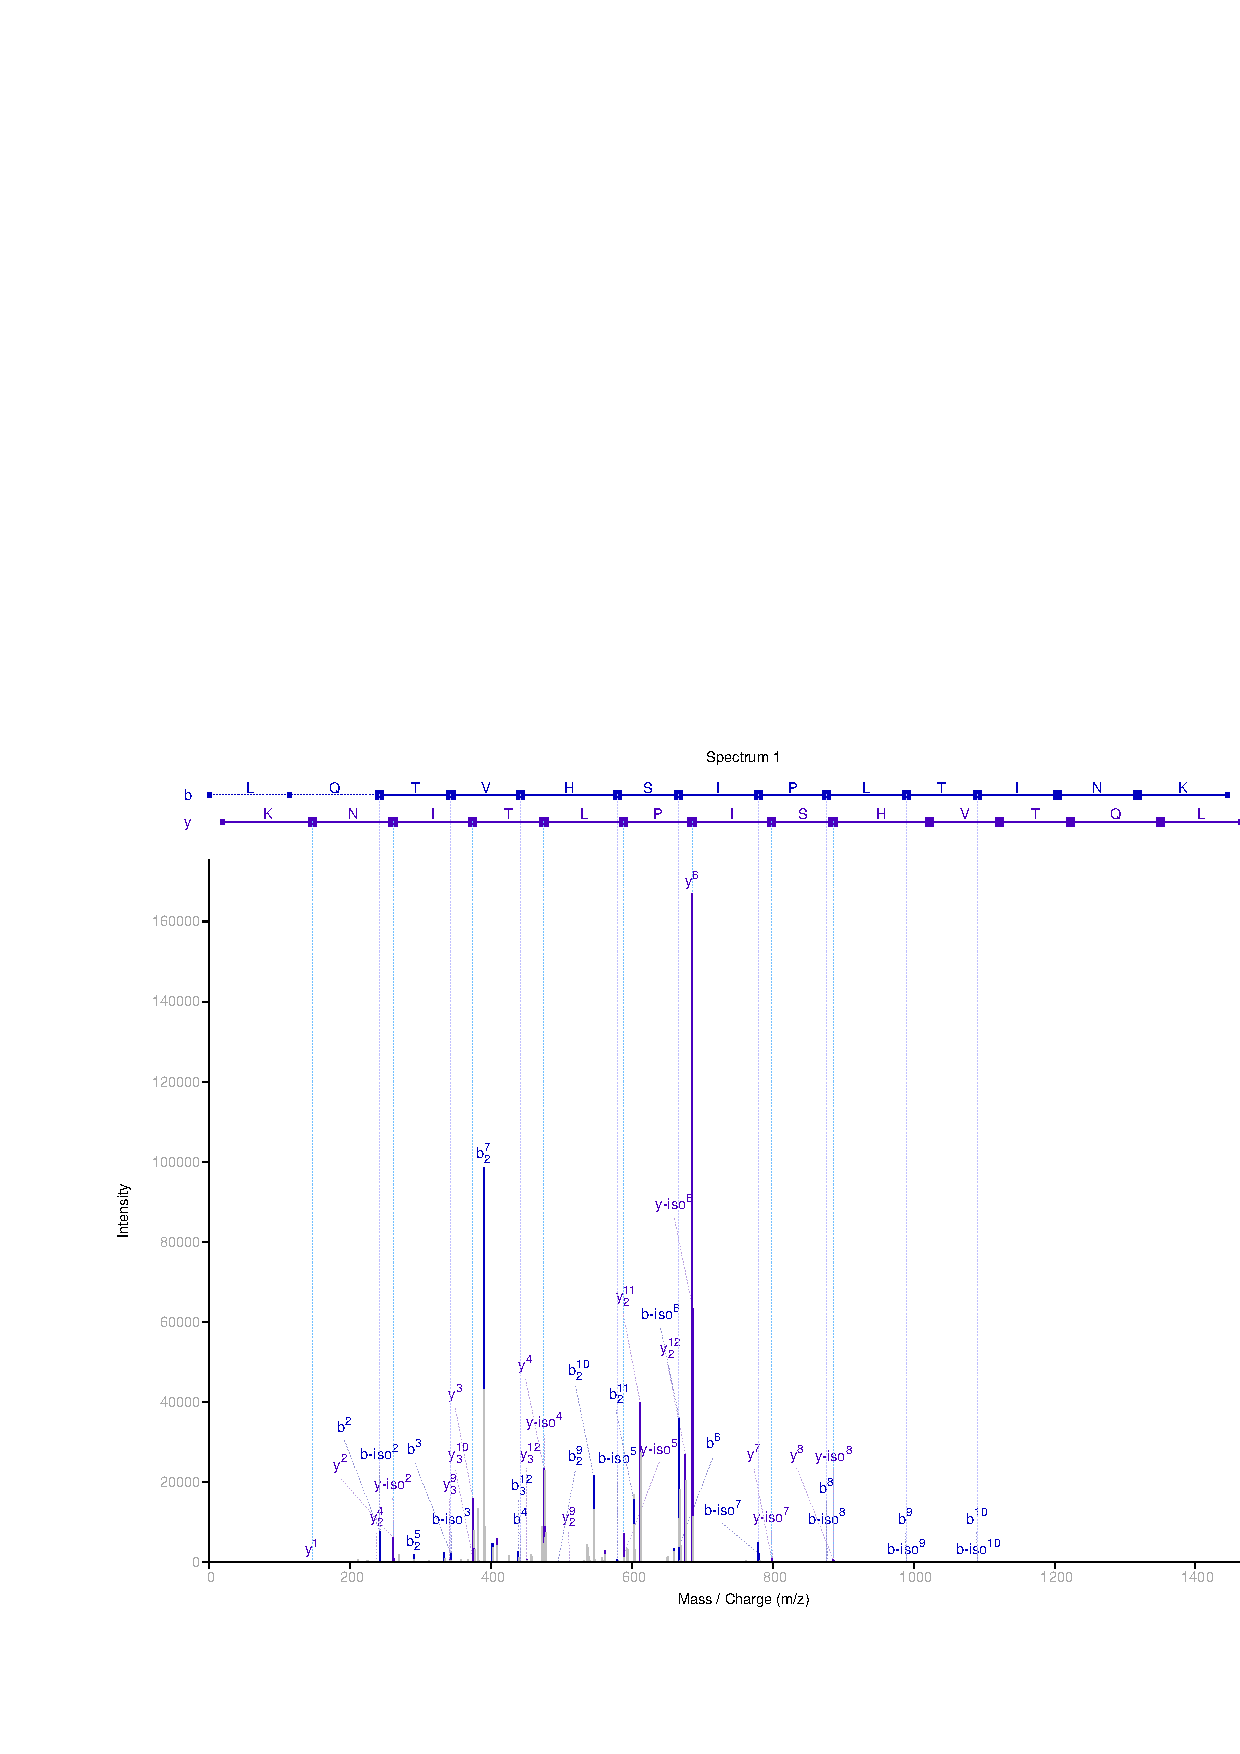
\includegraphics[scale=.37]{fig/synthetic/0055_LQ(T,-18)VHSIPLTINK_unmod.png}\\
b) \includegraphics[scale=.37]{fig/synthetic/0055_LQ(T,-18)VHSIPLTINK_mod1.png}
c) \includegraphics[scale=.37]{fig/synthetic/0055_LQ(T,-18)VHSIPLTINK_mod2.png}
\caption[Modification assignment comparison]{Comparison of unmodified and modified spectra with two possible modification assignments. Note that while phosphorylated fragments are labeled, they are not included in the LP score. a) Unmodified charge 3 spectrum used for LP b) Scan 975 from  ppeptidemix1\_CID\_Orbi.mgf with expected synthetic modification site c) Scan 975 from  ppeptidemix1\_CID\_Orbi.mgf with site assigned by LP}
\label{fig:charge3Incorrect}
\end{figure}  \clearpage
\setcounter{page}{1}
\setcounter{figure}{0}  % reset counter

\section{Supplemental results for the Lens dataset}

\begin{table}[h]
\centering
\caption{Lens Modifications}\label{tbl:lensModifications}
%\resizebox{7in}{!} {

\begin{tabular}{|l|l|l|}
\hline
$\delta$ Mass & Residues & Putative Modification \\
-18.010565 & D,E,S,T & Dehydration \\
-17.026549 & N, N-terminal Q & Succinimide, Gln $\rightarrow$ Pyro-glu \\
14.01565 & C,H,K & Methyl \\
15.994915 & H,M,W & Oxidataion \\
21.981943 & D,E & Sodiated \\
27.994915 & H,S,T & Formylation \\
28.031300 & K & Dimethylation \\
31.989829 & W & Dioxidation \\
39.994915 & N-terminal C & Pyro-carbamidomethyl \\
42.010565 & N-terminal, K & Acetylation \\
43.005814 & N-terminal, K & Carbamylation \\
43.989829 & W & Carboxylation \\ 
58.0361 & K	& Carboxymethyl \\
72.021129 & K & Carboxyethyl \\
79.966331 & S,T,Y & Phosphorylation \\
\hline
\end{tabular}
\end{table}

 \clearpage
%\setcounter{page}{1}
\setcounter{figure}{0}  % reset counter

\section{Supplemental results for the Yeast dataset}
\subsection{Results on unique MS3 -18 identifications}
\subsubsection{S,T, and Y are valid sites}

\begin{figure}[htbp]
\centering % trim=l b r t
\includegraphics[trim = 2mm 105mm 4mm 105mm,
clip,width=\textwidth]{fig/phospho/uniqueIds/size_dist_uniq_by_STY.pdf}
\caption{Distribution of number of variant groups, size of variant groups, and number of valid variants per valid group.}
\label{fig:yeast_sizedist_STY}
\end{figure}


\begin{table}[h]
  \centering
  \caption{Yeast MS3 dataset PTM site assignment FLR results on unique peptide identifications. At cosine score cutoff = $0.4$, $52$ cases rejected, $561$ cases accepted. S, T and Y are considered as valid sites.}\label{tbl:YeastFLR_uniq_STY}
\begin{tabular}{|c|l|l|l|l|l|}
\hline
Estimated Abundance & \multirow{2}{*}{FDR} & \multicolumn{4}{|c|}{\#Cases with k groups identified }\\
of Variant Group & & $k\ge 1$ & $k=1$ & $k=2$ & $k=3$\\
\hline
$\ge	60	\%$ &	0.02	\% &	91.8	\% &	91.8	\% &	0.0	\% &	0.0	\\
$\ge	55	\%$ &	0.02	\% &	94.1	\% &	94.1	\% &	0.0	\% &	0.0	\\
$\ge	50	\%$ &	0.03	\% &	95.1	\% &	94.9	\% &	0.2	\% &	0.0	\\
$\ge	45	\%$ &	0.03	\% &	96.2	\% &	95.6	\% &	0.6	\% &	0.0	\\
$\ge	40	\%$ &	0.03	\% &	96.8	\% &	94.9	\% &	1.9	\% &	0.0	\\
$\ge	35	\%$ &	0.04	\% &	97.9	\% &	95.1	\% &	2.8	\% &	0.0	\\
$\ge	34	\%$ &	0.04	\% &	97.9	\% &	94.9	\% &	3.0	\% &	0.0	\\
$\ge	33	\%$ &	0.04	\% &	98.3	\% &	94.9	\% &	3.4	\% &	0.0	\\
$\ge	32	\%$ &	0.05	\% &	98.3	\% &	94.9	\% &	3.4	\% &	0.0	\\
$\ge	31	\%$ &	0.05	\% &	98.3	\% &	94.7	\% &	3.6	\% &	0.0	\\
$\ge	30	\%$ &	0.05	\% &	98.5	\% &	94.7	\% &	3.8	\% &	0.0	\\
$\ge	25	\%$ &	0.06	\% &	98.9	\% &	93.7	\% &	4.9	\% &	0.2	\\
$\ge	20	\%$ &	0.08	\% &	99.1	\% &	92.8	\% &	6.1	\% &	0.2	\\
%$\ge	15	\%$ &	0.11	\% &	99.4	\% &	91.8	\% &	7.4	\% &	0.2	\\
%$\ge	10	\%$ &	0.16	\% &	99.6	\% &	90.1	\% &	8.9	\% &	0.6	\\
%$\ge	5	\%$ &	0.23	\% &	99.8	\% &	84.6	\% &	14.4	\% &	0.8	\\
\hline
\end{tabular}
\end{table}

\begin{figure}[htbp]
\centering % trim=l b r t
\includegraphics[trim = 0mm 90mm 20mm 90mm,clip,width=0.6\textwidth]{fig/phospho/uniqueIds/piechart_uniq_by_STY.pdf}
\caption{Yeast dataset results on unique MS3 -18 peptide identifications: Site assignment results for yeast dataset at $3\%$ FDR.}
\label{fig:yeast_piechart_uniqIds_STY}
\end{figure}

\clearpage
\subsubsection{S,T,Y,D, and E are valid sites}
\begin{figure}[htbp]
\centering % trim=l b r t
\includegraphics[trim = 2mm 105mm 4mm 105mm,
clip,width=\textwidth]{fig/phospho/uniqueIds/size_dist_uniq_by_STYDE.pdf}
\caption{Distribution of number of variant groups, size of variant groups, and number of valid variants per valid group.}
\label{fig:yeast_sizedist_STYDE}
\end{figure}

\begin{table}[h]
  \centering
  \caption{Yeast MS3 dataset PTM site assignment FLR results on unique peptide identifications. At cosine score cutoff = $0.4$, $52$ cases rejected, $561$ cases accepted. S, T, Y, D and E are considered as valid sites.}\label{tbl:YeastFLR_uniq_STYDE}
\begin{tabular}{|c|l|l|l|l|l|l|}
\hline
Estimated Abundance & \multirow{2}{*}{FDR} & \multicolumn{5}{|c|}{\#Cases with k groups identified }\\
of Variant Group & & $k\ge 1$ & $k=1$ & $k=2$ & $k=3$  & $k=4$\\
\hline
$\ge	60	\%$ &	0.01	\% &	90.6	\% &	90.6	\% &	0.0	\% &	0.0	\% &	0.0	\\
$\ge	55	\%$ &	0.02	\% &	92.7	\% &	92.7	\% &	0.0	\% &	0.0	\% &	0.0	\\
$\ge	50	\%$ &	0.02	\% &	93.6	\% &	93.4	\% &	0.2	\% &	0.0	\% &	0.0	\\
$\ge	45	\%$ &	0.02	\% &	94.3	\% &	93.8	\% &	0.5	\% &	0.0	\% &	0.0	\\
$\ge	40	\%$ &	0.02	\% &	94.8	\% &	92.7	\% &	2.1	\% &	0.0	\% &	0.0	\\
$\ge	35	\%$ &	0.03	\% &	95.7	\% &	92.3	\% &	3.4	\% &	0.0	\% &	0.0	\\
$\ge	30	\%$ &	0.03	\% &	96.4	\% &	91.6	\% &	4.8	\% &	0.0	\% &	0.0	\\
$\ge	25	\%$ &	0.04	\% &	96.6	\% &	89.7	\% &	6.8	\% &	0.2	\% &	0.0	\\
$\ge	20	\%$ &	0.05	\% &	96.6	\% &	86.8	\% &	9.4	\% &	0.4	\% &	0.0	\\
%$\ge	15	\%$ &	0.05	\% &	97.0	\% &	84.1	\% &	11.8	\% &	1.1	\% &	0.0	\\
%$\ge	10	\%$ &	0.06	\% &	97.0	\% &	78.3	\% &	16.8	\% &	1.6	\% &	0.4	\\
%$\ge	5	\%$ &	0.10	\% &	97.1	\% &	71.1	\% &	22.1	\% &	3.4	\% &	0.5	\\
\hline
\end{tabular}
\end{table}

\begin{figure}[htbp]
\centering % trim=l b r t
\includegraphics[trim = 0mm 90mm 20mm 90mm,clip,width=0.6\textwidth]{fig/phospho/uniqueIds/piechart_uniq_by_STYDE.pdf}
\caption{Yeast dataset results on unique MS3 -18 peptide identifications: Site assignment results for yeast dataset at $2\%$ FDR.}
\label{fig:yeast_piechart_uniqIds_STYDE}
\end{figure}

\clearpage
\subsubsection{Phosphate Localization Score (PLS)}
\begin{figure}[htbp]
\centering % trim=l b r t
\includegraphics[trim = 0mm 90mm 20mm 90mm,clip,width=0.6\textwidth]{fig/phospho/uniqueIds/PLS_figs/uniqIds_PLS_histogram.pdf}
\caption{Yeast dataset results on unique MS3 -18 peptide identifications: Histogram of PLS. $38\%$ of the PLS scores are $\ge 19$ and $51\%$ are $\ge 13$.}
\label{fig:yeast_pls}
\end{figure}

\begin{figure}[htbp]
\centering % trim=l b r t
\includegraphics[trim = 0mm 90mm 20mm 90mm,clip,width=0.6\textwidth]{fig/phospho/uniqueIds/PLS_figs/uniqIds_PLS_by_num_valid_sites.pdf}
\caption{Yeast dataset results on unique MS3 -18 peptide identifications: Distribution of PLS by the number of valid sites (S, T, Y) in the peptide.}
\label{fig:yeast_pls}
\end{figure}

\begin{figure}[htbp]
\centering % trim=l b r t
\includegraphics[trim = 0mm 90mm 20mm 90mm,clip,width=\textwidth]{fig/phospho/uniqueIds/PLS_figs/uniqIds_PLS_hist_by_num_valid_sites.pdf}
\caption{Yeast dataset results on unique MS3 -18 peptide identifications: Histogram of PLS by the number of valid sites (S, T, Y) in the peptide.}
\label{fig:yeast_pls}
\end{figure}

\begin{figure}[htbp]
\centering % trim=l b r t
\includegraphics[trim = 0mm 90mm 20mm 90mm,clip,width=0.6\textwidth]{fig/phospho/uniqueIds/PLS_figs/uniqIds_PLS_by_valid_site_distance.pdf}
\caption{Yeast dataset results on unique MS3 -18 peptide identifications: PLS by the distance between the closest two valid sites in the peptide.}
\label{fig:yeast_pls}
\end{figure}


\clearpage
\subsection{Results on all MS3 -18 identifications}

\subsubsection{S,T, and Y are valid sites}

\begin{figure}[htbp]
\centering % trim=l b r t
\includegraphics[trim = 2mm 105mm 4mm 105mm,
clip,width=\textwidth]{fig/phospho/allIds/size_dist_all_by_STY.pdf}
\caption{Yeast results on all ids: Distribution of number of variant groups, size of variant groups, and number of valid variants per valid group.}
\label{fig:yeast_sizedist_STY}
\end{figure}


\begin{table}[h]
  \centering
  \caption{Yeast MS3 dataset PTM site assignment FLR results on all peptide identifications. At cosine score cutoff = $0.4$, $277$ cases rejected, $2251$ cases accepted. S, T and Y are considered as valid sites.}\label{tbl:YeastFLR_all_STY}
\begin{tabular}{|c|l|l|l|l|l|}
\hline
Estimated Abundance & \multirow{2}{*}{FDR} & \multicolumn{4}{|c|}{\#Cases with k groups identified }\\
of Variant Group & & $k\ge 1$ & $k=1$ & $k=2$ & $k=3$\\
\hline
$\ge	60	\%$ &	0.05	\% &	90.3	\% &	90.3	\% &	0.0	\% &	0.0	\\
$\ge	55	\%$ &	0.06	\% &	91.5	\% &	91.5	\% &	0.0	\% &	0.0	\\
$\ge	50	\%$ &	0.06	\% &	92.5	\% &	92.5	\% &	0.0	\% &	0.0	\\
$\ge	45	\%$ &	0.06	\% &	93.4	\% &	93.2	\% &	0.2	\% &	0.0	\\
$\ge	40	\%$ &	0.07	\% &	93.8	\% &	93.2	\% &	0.6	\% &	0.0	\\
$\ge	35	\%$ &	0.08	\% &	94.2	\% &	93.3	\% &	0.9	\% &	0.0	\\
$\ge	30	\%$ &	0.09	\% &	94.4	\% &	92.9	\% &	1.5	\% &	0.0	\\
$\ge	25	\%$ &	0.11	\% &	94.8	\% &	92.4	\% &	2.4	\% &	0.0	\\
$\ge	20	\%$ &	0.14	\% &	94.9	\% &	91.4	\% &	3.3	\% &	0.1	\\
$\ge	15	\%$ &	0.17	\% &	95.4	\% &	90.3	\% &	4.9	\% &	0.1	\\
%$\ge	10	\%$ &	0.23	\% &	95.8	\% &	87.9	\% &	7.5	\% &	0.4	\\
%$\ge	5	\%$ &	0.30	\% &	96.5	\% &	83.0	\% &	12.9	\% &	0.6	\\

\hline
\end{tabular}
\end{table}

\begin{figure}[htbp]
\centering % trim=l b r t
\includegraphics[trim = 0mm 90mm 20mm 90mm,clip,width=0.6\textwidth]{fig/phospho/allIds/piechart_all_by_STY.pdf}
\caption{Yeast dataset results on unique MS3 -18 peptide identifications: Site assignment results for yeast dataset at $3\%$ FDR.}
\label{fig:yeast_piechart_uniqIds_STY}
\end{figure}

\clearpage
\subsubsection{S,T,Y,D, and E are valid sites}
\begin{figure}[htbp]
\centering % trim=l b r t
\includegraphics[trim = 2mm 105mm 4mm 105mm,
clip,width=\textwidth]{fig/phospho/allIds/size_dist_all_by_STYDE.pdf}
\caption{Yeast results on all ids: Distribution of number of variant groups, size of variant groups, and number of valid variants per valid group.}
\label{fig:yeast_sizedist_STYDE}
\end{figure}

\begin{table}[h]
  \centering
  \caption{Yeast MS3 dataset PTM site assignment FLR results on all peptide identifications. At cosine score cutoff = $0.4$, $277$ cases rejected, $2251$ cases accepted. S, T, Y, D and E are considered as valid sites.}\label{tbl:YeastFLR_all_STYDE}
\begin{tabular}{|c|l|l|l|l|l|l|}
\hline
Estimated Abundance & \multirow{2}{*}{FDR} & \multicolumn{5}{|c|}{\#Cases with k groups identified }\\
of Variant Group & & $k\ge 1$ & $k=1$ & $k=2$ & $k=3$  & $k=4$\\
\hline
$\ge	60	\%$ &	0.05	\% &	90.8	\% &	90.8	\% &	0.0	\% &	0.0	\% &	0.0	\\
$\ge	55	\%$ &	0.06	\% &	92.0	\% &	92.0	\% &	0.0	\% &	0.0	\% &	0.0	\\
$\ge	50	\%$ &	0.06	\% &	93.2	\% &	92.9	\% &	0.2	\% &	0.0	\% &	0.0	\\
$\ge	45	\%$ &	0.06	\% &	94.0	\% &	93.4	\% &	0.5	\% &	0.0	\% &	0.0	\\
$\ge	40	\%$ &	0.06	\% &	94.6	\% &	93.3	\% &	1.2	\% &	0.0	\% &	0.0	\\
$\ge	35	\%$ &	0.07	\% &	95.1	\% &	93.2	\% &	1.9	\% &	0.0	\% &	0.0	\\
$\ge	30	\%$ &	0.07	\% &	95.6	\% &	92.8	\% &	2.8	\% &	0.0	\% &	0.0	\\
$\ge	25	\%$ &	0.08	\% &	96.5	\% &	91.9	\% &	4.5	\% &	0.1	\% &	0.0	\\
$\ge	20	\%$ &	0.08	\% &	97.5	\% &	90.6	\% &	6.6	\% &	0.3	\% &	0.0	\\
$\ge	15	\%$ &	0.10	\% &	98.5	\% &	88.1	\% &	9.6	\% &	0.8	\% &	0.0	\\
%$\ge	10	\%$ &	0.12	\% &	99.2	\% &	82.7	\% &	15.0	\% &	1.4	\% &	0.1	\\
%$\ge	5	\%$ &	0.15	\% &	99.6	\% &	74.3	\% &	21.6	\% &	3.4	\% &	0.2	\\
\hline
\end{tabular}
\end{table}

\begin{figure}[htbp]
\centering % trim=l b r t
\includegraphics[trim = 0mm 90mm 20mm 90mm,clip,width=0.6\textwidth]{fig/phospho/allIds/piechart_all_by_STYDE.pdf}
\caption{Yeast dataset results on unique MS3 -18 peptide identifications: Site assignment results for yeast dataset at $2\%$ FDR.}
\label{fig:yeast_piechart_uniqIds_STYDE}
\end{figure}

\clearpage
\subsubsection{Phosphate Localization Score (PLS)}
\begin{figure}[htbp]
\centering % trim=l b r t
\includegraphics[trim = 0mm 90mm 20mm 90mm,clip,width=0.6\textwidth]{fig/phospho/allIds/PLS_figs/allIds_PLS_histogram.pdf}
\caption{Yeast dataset results on all MS3 -18 peptide identifications: Histogram of PLS. $38\%$ of the PLS scores are $\ge 19$ and $51\%$ are $\ge 13$.}
\label{fig:yeast_pls}
\end{figure}

\begin{figure}[htbp]
\centering % trim=l b r t
\includegraphics[trim = 0mm 90mm 20mm 90mm,clip,width=0.6\textwidth]{fig/phospho/allIds/PLS_figs/allIds_PLS_by_num_valid_sites.pdf}
\caption{Yeast dataset results on all MS3 -18 peptide identifications: Distribution of PLS by the number of valid sites (S, T, Y) in the peptide.}
\label{fig:yeast_pls}
\end{figure}

\begin{figure}[htbp]
\centering % trim=l b r t
\includegraphics[trim = 0mm 90mm 20mm 90mm,clip,width=\textwidth]{fig/phospho/allIds/PLS_figs/allIds_PLS_hist_by_num_valid_sites.pdf}
\caption{Yeast dataset results on all MS3 -18 peptide identifications: Histogram of PLS by the number of valid sites (S, T, Y) in the peptide.}
\label{fig:yeast_pls}
\end{figure}

\begin{figure}[htbp]
\centering % trim=l b r t
\includegraphics[trim = 0mm 90mm 20mm 90mm,clip,width=0.6\textwidth]{fig/phospho/allIds/PLS_figs/allIds_PLS_by_valid_site_distance.pdf}
\caption{Yeast dataset results on all MS3 -18 peptide identifications: PLS by the distance between the closest two valid sites in the peptide.}
\label{fig:yeast_pls}
\end{figure}

 \clearpage


%\section{Appendix}
%\subsection{Inspect Search Parameters Used}
%Database: XXXX
%Instrument,ESI-ION-TRAP\\
%Protease, Trypsin\\
%Parent mass tolerance, 2.000000 Daltons\\
%Ion tolerance, 0.500000 Daltons\\
%Maximum number of PTM allowed per peptide, 1\\
%PTM, delta mass: +15.999400 Da, affected: MW, type: opt\\
%PTM, delta mass: -17.030500 Da, affected: Q, type: nterminal\\
%PTM, delta mass: +43.024700 Da, affected: *, type: nterminal\\
%PTM, delta mass: 42 Da, affected: *, type: nterminal\\
%PTM, delta mass: 28 Da, affected: SH, type: opt\\
%PTM, delta mass: 28 Da, affected: *, type: nterminal\\
%Sequence, sprot.ALL.20070802\\
%Results were filtered at a spectrum-level p-value of $0.01$, measured by hits to the decoy database\\

\end{document} 